\chapter{JT60-SA control design}

\section{Machine description}

JT60-SA is an under-construction superconductive tokamak located at one of the facilities from the National Institutes for Quantum and Radiological Science and Technology (QST)  at  Naka, Japan whose principal purpose is  the contribution to early realization of fusion energy by supporting the exploitation and resolving key physics for the ITER reactor. Figure ~\ref{JT60schm} shows the overall general configuration and the most remarkable elements of the machine. The JT-60SA  vacuum chamber will have a major radius of 2.96~ m and a Minor radius of 1.18~ m with an overall plasma volume of 132~ $m^3$ ~\cite{Spears2014} .
\smallskip

\begin{figure}[h]
	\centering
	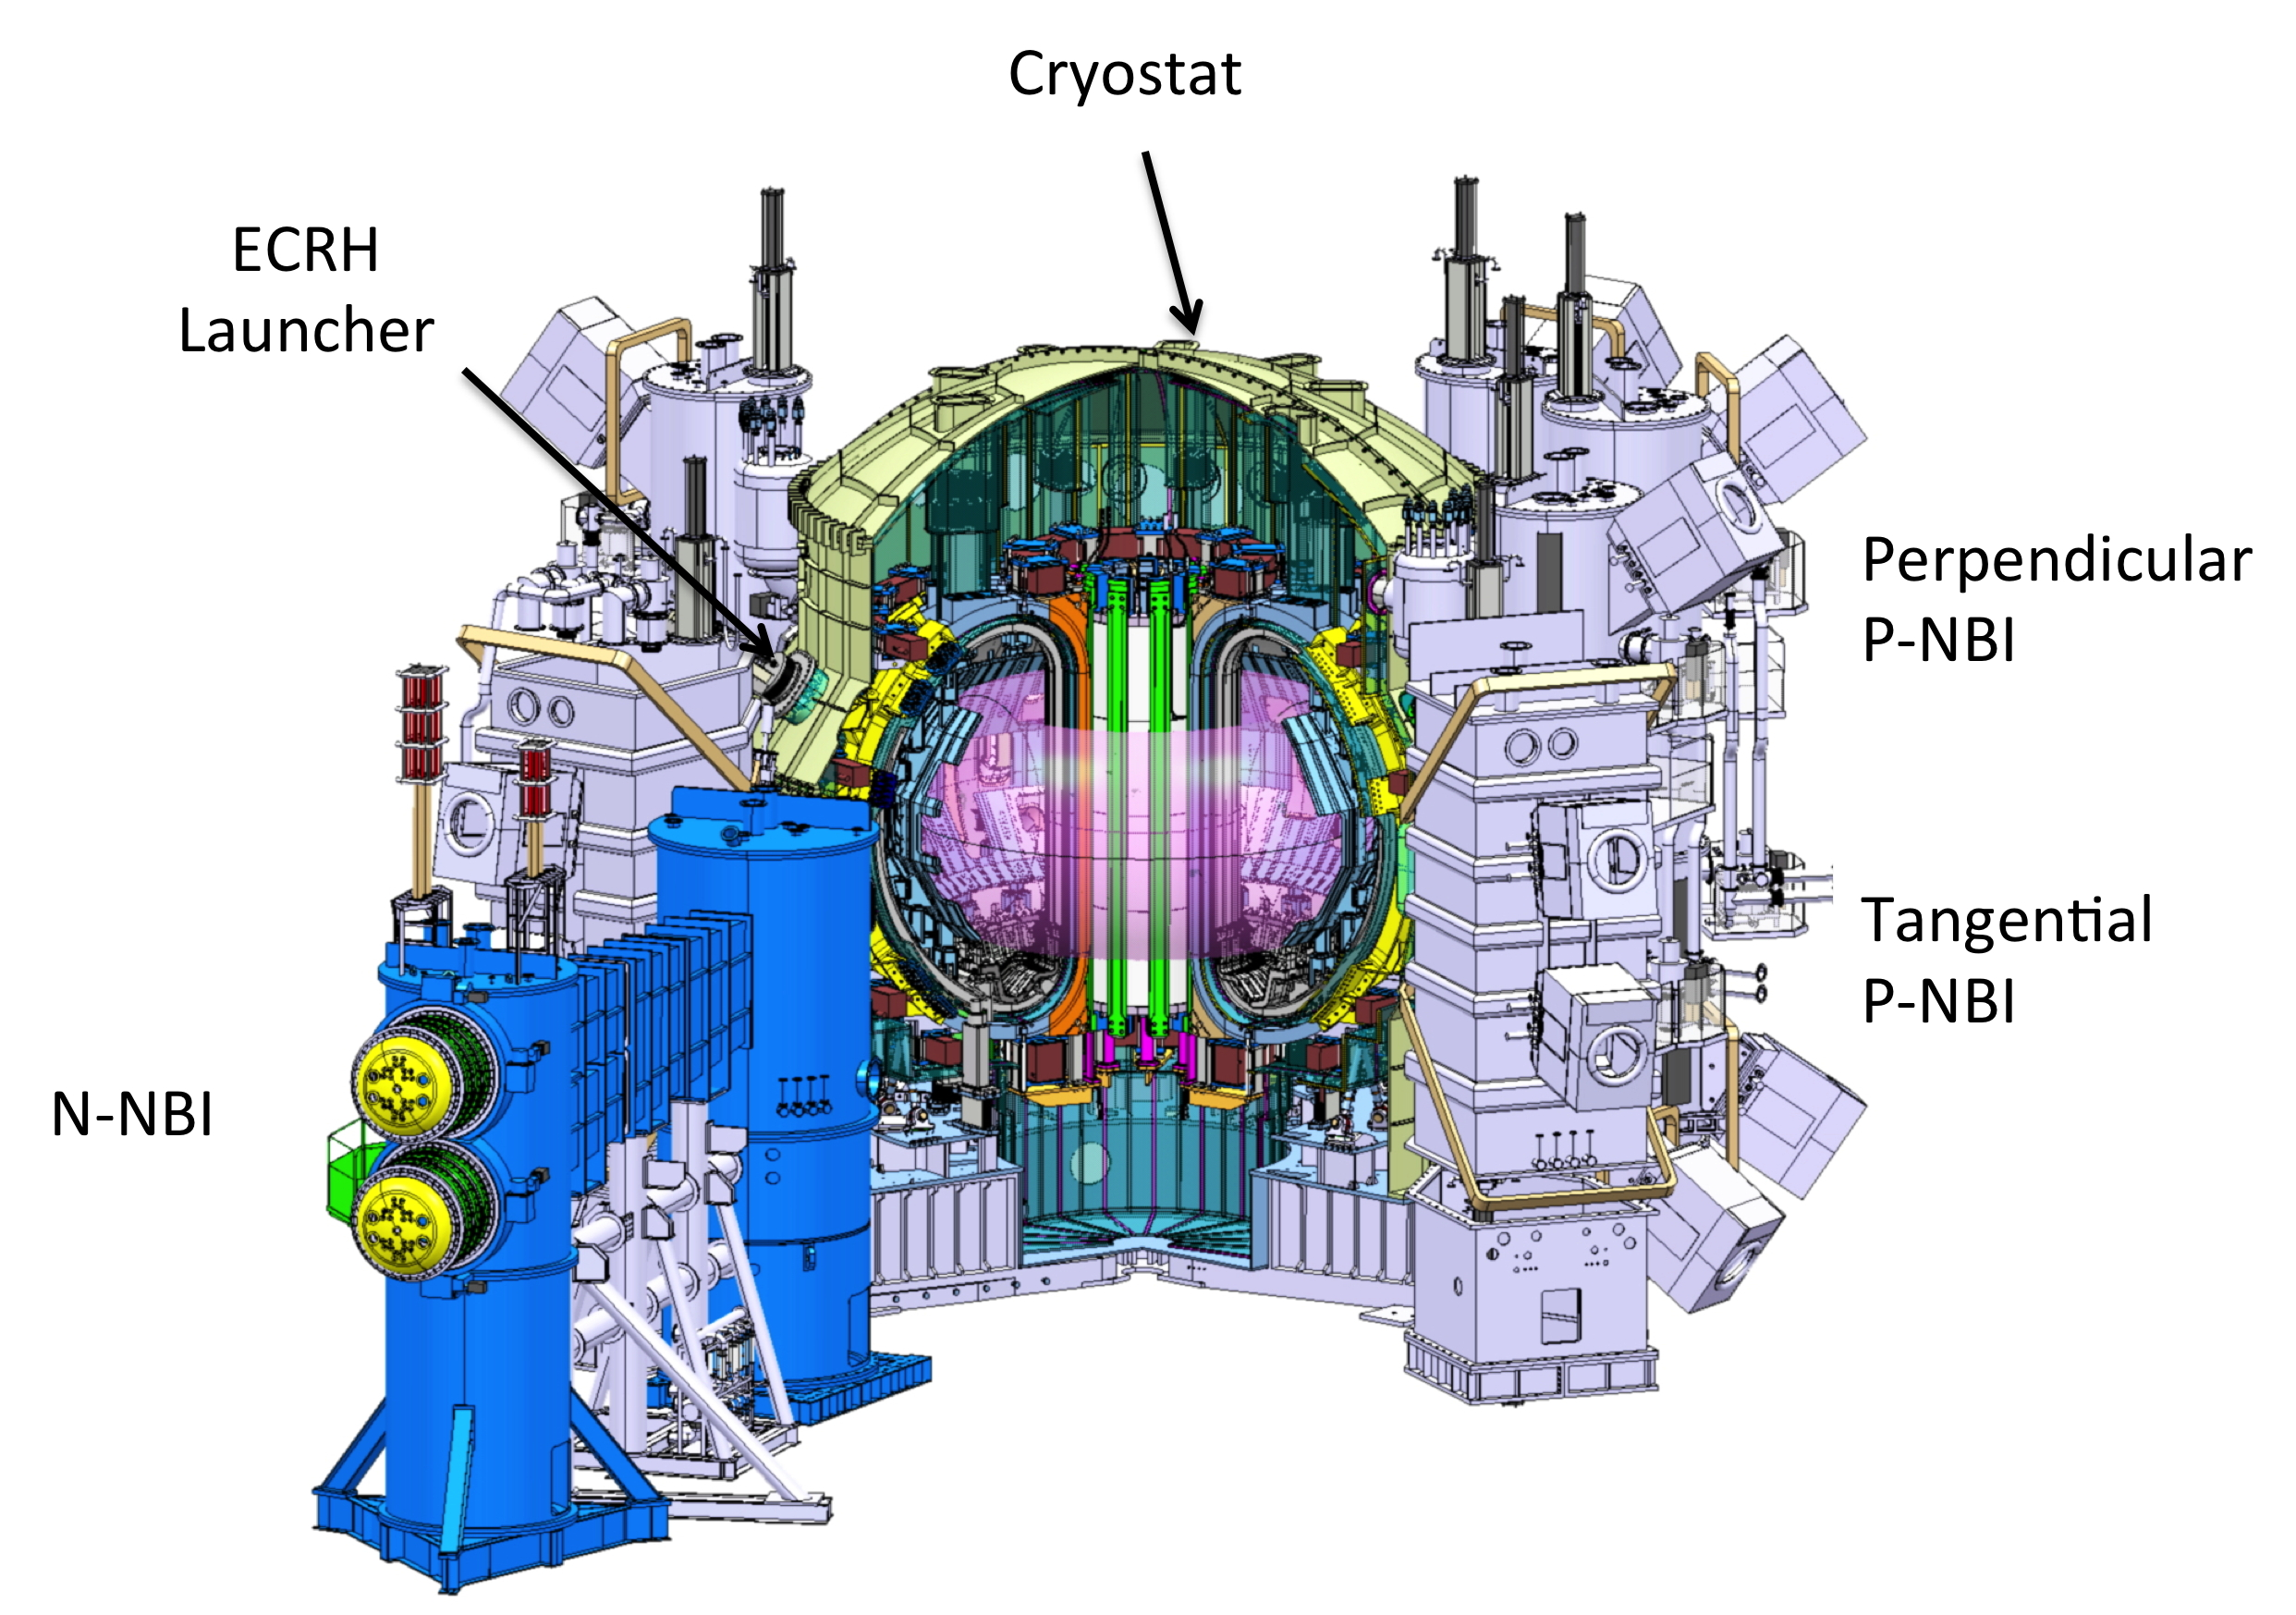
\includegraphics[width=0.75\textwidth]{Chp3/JT60SA.png}
	
	\caption{\label{JT60schm}JT60-SA tokamak configuration and its main elements ~\cite{JT60SA:ResearchPlan}.}
\end{figure}

The Poloidal Field (PF) coils shown in JT60-SA cross-section from figure ~\ref{JT60coils} consist of two sets of superconductive coils: the Equilibrium Field Coils (EF1–6) and the Central Solenoid (consisting of four independent coils, named CS1–4). Furthermore, two in-vessel Fast Plasma Position Copper Coils (FPPC1–2) will also be installed ~\cite{NCruz}.The total of 12 PF coils have independent power sources for the control of the plasma current, position and shape.   
\smallskip

\begin{figure}
	\centering
	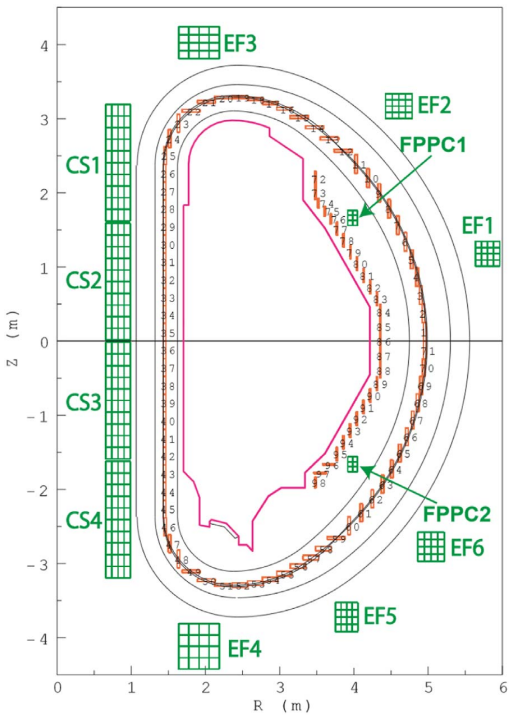
\includegraphics[width=0.55\textwidth]{Chp3/JT60Coils.png}

	\caption{	\label{JT60coils}JT-60SA poloidal cross-section and layout of the Poloidal Field coils system ~\cite{NCruz}.}
\end{figure}

JT-60SA shall be capable of investigating different design scenarios. As refereed  in 
~\cite{JT60SA:PID} it exists a set of 6 reference scenarios, additional ones, including some with a shorter repetition rate will be defined in future. For the control study in this section all simulations will be built based on the Scenario~2 characteristics. In particular, Scenario~2 refers to a~5.5 MA inductive lower single null discharge. The Scenario~2 its divided in 5 time snapshots with different equilibrium each one starting at  t=-40~s until t= 177.96~s. The different Last Closed Flux Surfaces (LCFS) for each time window are shown in figure~\ref{Scen2}, the time sequence starts at the X-point formation (XPF)	followed by the Start of Heating(SOH), the Start of Flattop (SOF), End of Flattop (EOF), End Of Cooling(EOC) and finishing with the End of Currents in the PF coils (EOC). In this section, reconstruction methods and control algorithms will be based on the \emph{Start of Flattop}~(SOF) equilibrium shown in figure~\ref{SOF}. The nominal values for the plasma current, the poloidal beta and the internal inductance for Scenario~2 at SOF are~$I_{p_{eq}}~=~5.5$~MA,~ $\beta_{p_{eq}}=0.53$, and~$l_{i_{eq}}=0.85$.\smallskip

\begin{figure}[h]
	\centering
	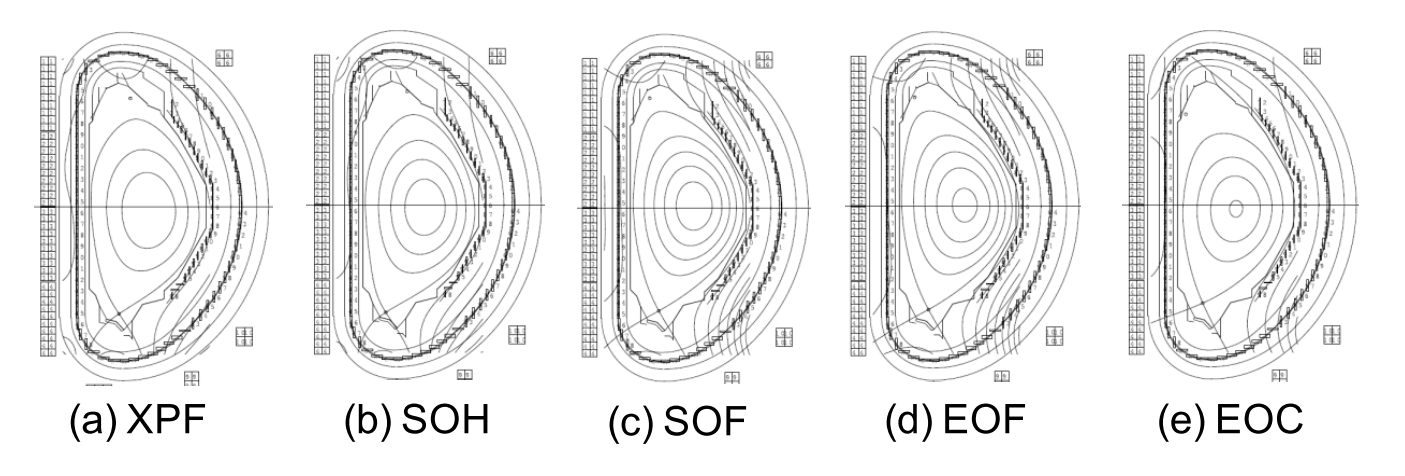
\includegraphics[width=0.99\textwidth]{Chp3/scenario2SnapShots.png}
	
	\caption{LCFS Equilibria corresponding to the different Scenario~2 snapshots:  X-point formation (XPF), Start of Heating(SOH), the Start of Flattop (SOF), End of Flattop (EOF), End Of Cooling(EOC) and  End of Currents in the PF coils (EOC) ~\cite{JT60SA:PID}. \label{Scen2}}
\end{figure}


\begin{figure}[h]
	\centering
	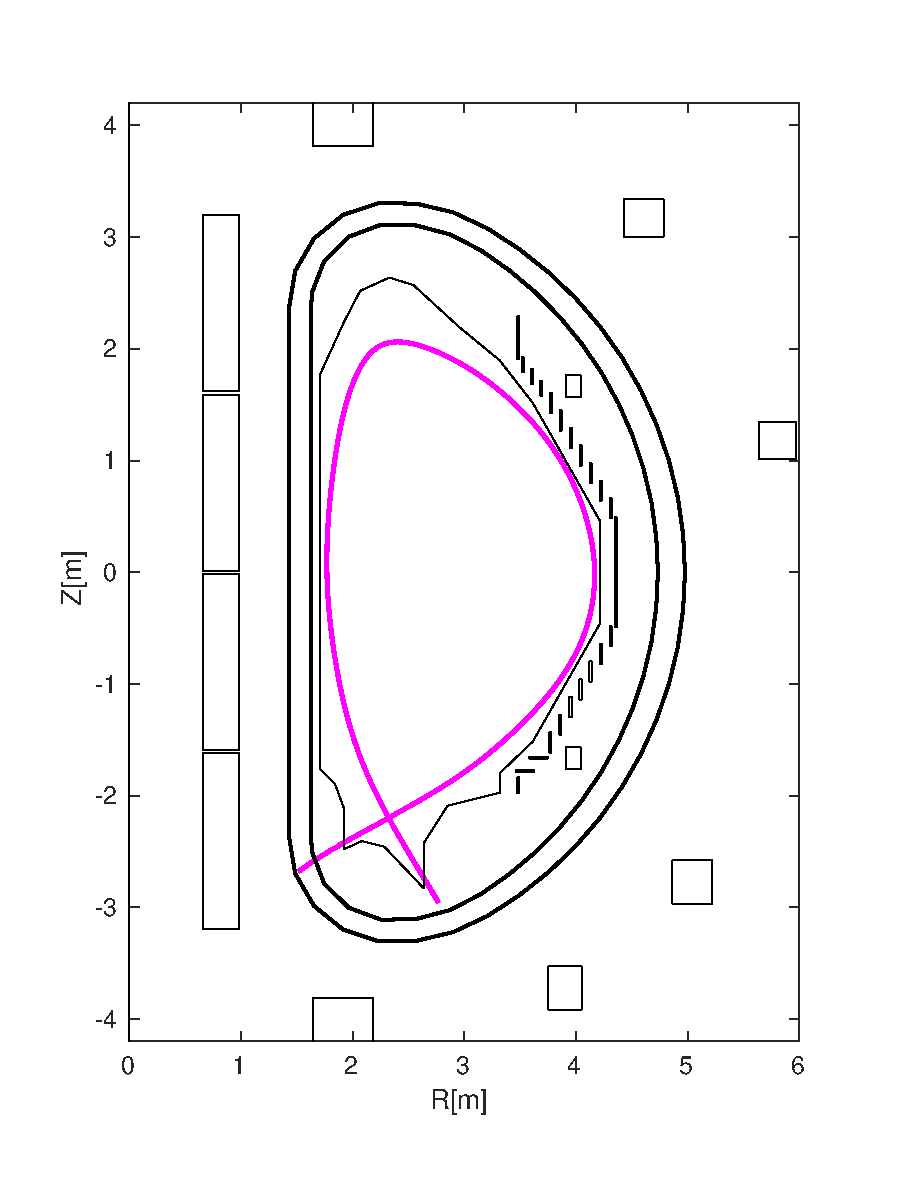
\includegraphics[width=0.5\textwidth]{Chp3/scenario2_SOF.eps}
	
	\caption{Poloidal cross-section of the JT-60SA plasma at the Start of the Flat Top~(SOF) for reference Scenario~2. At SOF, the nominal plasma current is ~5.5~MA, while the nominal values for poloidal beta~$\beta_p$ and internal inductance~$l_i$ are~0.53 and~0.85, respectively.	\label{SOF}}
\end{figure}



This chapter will address two different approaches for the LCFS reconstruction along  with different plasma current, shape and position controllers for JT60-SA in order to achieve and maintain the desired operational scenario given the plasma equilibrium in the SOF while the performance of the controllers is compared .



\section{CREATE magnetic reconstruction tools}

CREATE-NL (Consorzio di Ricerca per l' Energia, l' Automazione e le Tecnologie dell' Elettromagnetismo) is a finite elements method (FEM\footnote{It is well known that many physical and engineering systems are expressed in terms of partial differential equations which cannot be solved via analytical methods. One of the most recurrent techniques is numerical discretization to approximate the solution of the partial differential equations, the FEM is commonly used to solve these approximations in two or three space variables, in this particular case for a numerical solution of the well-known Grad-Shafranov equation. }) solver implemented on \textsc{Matlab}. It deals with the free boundary dynamic plasma equilibrium problem i.e. the MHD (Magneto-Hydro-Dynamics) time evolution of 2D axisymmetric plasmas in tokamaks, including eddy currents in the passive structures, and feedback control laws for current, position and shape control ~\cite{Albanese:CREATENLnew}.
\smallskip

Using the CREATE codes~\cite{Albanese:CREATEL,Albanese:CREATENLnew} it is possible to retrieve a linearized state-space model that describes the plasma magnetic behavior around that equilibrium\footnote{Reference  ~\cite[Sec.~3]{NCruz} can be consulted for more details about the use of the CREATE equilibrium codes to retrieve plasma linearized models.}.It should be noted that CREATE-NL equilibrium solver has been validated on several tokamaks such as JET and EAST. A JT60-SA CREATE-NL electromagnetic linear model around the equilibrium from the Scenario~2-~SOF  for the plasma-circuit response has been used for  designing  the controller presented in next section.
\smallskip






\section{Controller design}

The JET (Joint European Torus) tokamak was the first machine where around 2005 a new model based plasma current and shape controller was set up and tested  with the existing active circuits and control hardware. The novelty controller was the eXtreme Shape Controller (XSC) and its aim was to improve  the performance of the, back then, present controller to allow the control of extremely shaped plasmas with higher values of elongation and triangularity ~\cite{Albanese2005}. More recently this control approach was utilized at TCV ~\cite{anand2017novel}. At JET, the XSC recently enabled the control of high triangularity shapes with both strike points in the divertor corner, which has a large impact in the H-mode confinement in the case of the ITER-like wall at JET~\cite{de2016recent}.   
 \smallskip
 
 Usually the controlled shape geometrical descriptors are the distances between the plasma boundary and the vessel at some specific points. These plasma-wall distances are called gaps ~\cite{Ambrosino:TCST2008}. The gaps are segments that can be used to describe the shape of the plasma boundary. Being~$g_i$ the abscissa along the~$i$-th control segment, we assume that~$g_i=0$ at the first wall. \emph{Gap-based} plasma shape control is achieved by controlling to zero the difference $g_{i_{ref}}-g_i$ on a sufficiently large number of gaps, being~$g_{i_ref}$ the value of the abscissa on the~$i$-th control segment for the reference shape. Figure ~\ref{figure:85_gaps} shows a poloidal cross-section of JT-60SA together with a set of 85 gaps used for the assessment of the plasma shape control.
 \smallskip
 
 \begin{figure}[h]
 	\begin{center}
 		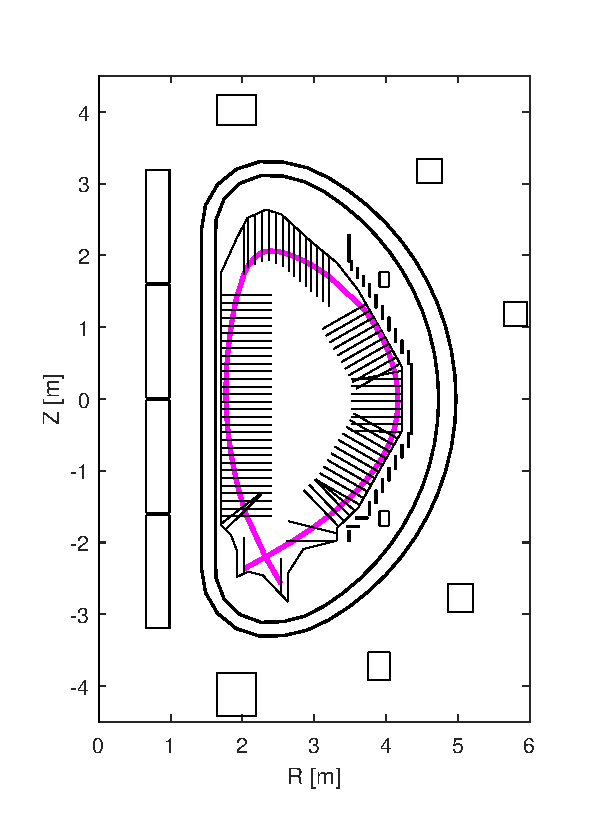
\includegraphics[width=0.45\textwidth]{Chp3/85_gaps_2.eps}
 	\end{center}\caption{Poloidal cross-section of the JT-60SA plasma at the Start of the Flat Top~(SOF) for reference Scenario~2. At SOF, the nominal plasma current is~5.5~MA, while the nominal values for poloidal beta~$\beta_p$ and internal inductance~$l_i$ are~0.53 and~0.85, respectively. In this figure the~85 gaps used to assess the plasma shape controller performance are shown.}\label{figure:85_gaps}
 \end{figure}
 
  The XSC algorithm can be used either to implement a gap-based control strategy, or an isoflux one, as it has been proposed in ~\cite{NCruz}. The isoflux strategy consists in controlling the X-point position along with a set of flux differences between the flux at some selected control points along the desired plasma boundary and the X-point flux. Thus the XSC block inputs are the error between the X-point flux and the fluxes in the control points, and the X-point position error.
\smallskip


The peculiarity of the XSC approach is that it permits to control a number of plasma shape descriptors that is greater than the number of available actuators, i.e. of PF Circuits, this  is basically tackled by using a singular value decomposition (SVD) to identify the principal directions of the algebraic mapping between coil currents and geometrical descriptors ~\cite{Albanese2005}. The XSC control relies on the PFC decoupling controller (more details can be found in~\cite[Section~4.4]{NCruz}), since it is assumed that each~PF coil can be treated as an independent single-input-single-output (SISO) channel whose dynamic response is modeled in the Laplace domain by
\[
I_{PF_i}(s) = \frac{I_{PF_{ref\,,i}}(s)}{1+s\tau_{PF}}\,,
\]
where~$I_{PF_i}$ and~$I_{PF_{ref_i}}$ are the Laplace transform of the measured and reference current in the~$i$-th PFC, respectively, and where it is assumed that all the PFC exhibit the same bandwidth (i.e.,~they have the same time constant~$\tau_{PF}$).
\smallskip

Denoting by~$\delta Y(s)$ the Laplace transform of the variations of the~$n_G$ shape descriptors  to be controlled, it is possible to exploit the CREATE electromagnetic linear model~\cite{NCruz} that links the variation of the PFC reference currents~$\delta I_{PF_{ref}}$ to ~$\delta Y(s)$, i.e.
\[
\delta Y(s) = C\frac{\delta I_{PF_{ref}}(s)}{1+s\tau_{PF}}\,,
\]
which, at steady-state, implies~ $\delta Y(s) = C \delta I_{PF_{ref}}(s)$.

If the number of controlled plasma shape descriptors~$n_G$ is such that~$n_G~>~n_{PF}$, the XSC computes the additional current references as
\begin{equation}\label{equation:XSC_new}
\delta I_{PF_{ref}}=C^\dag\delta Y\,.
\end{equation}
where the matrix~$C^\dag$ denotes the pseudo-inverse of~$C$\footnote{$C$ ~ is the output matrix from the state-space linearized CREATE model for JT60-SA.} that can be computed via the singular value decomposition (SVD). As a result, the XSC algorithm minimizes the following steady-state performance index
\begin{equation}\label{equation:XSCcost}
J_{XSC} = \lim_{t\to +
	\infty}(\delta Y_{ref}-\delta Y(t))^T(\delta Y_{ref}-\delta Y(t))\,,
\end{equation}
where~$\delta Y_{ref}$ are constant references for the geometrical descriptors. When the SVD of the~$C$ matrix is used to minimize~\eqref{equation:XSCcost}, it may happen that some singular values (depending on the plasma configuration) are one order of magnitude smaller than the others. This fact implies that minimizing the performance index~\eqref{equation:XSCcost} retaining all the singular values results in a large control effort at the steady-state, that is a large request on some PFC currents which have only a minor effect on the plasma shape. In order to minimize also the control effort, the additional references~\eqref{equation:XSC_new} are generated by using only the~$\bar{n}<n_{PF}$ linear combinations of PF currents which are related to the largest singular values of the~$C$ matrix. This is achieved by using only the~$\bar{n}$ singular values when computing the pseudo-inverse~$C^\dag$.
\smallskip

Moreover, the PFC current variations given by~\eqref{equation:XSC_new} are summed to the scenario currents and sent to the PFC decoupling controller as references to be tracked. It is worth to remark here that the dynamnic behavior of the XSC is improved by adding a set of proportional-integral-derivative (PID) controllers on each PF coil channel (see~\cite{Ariola:XSC} for a complete description of the XSC control scheme).
\smallskip

For the development of this work both approaches of the XSC strategy were studied and simulated for a different number of control points: isoflux and gap-based controllers. In addition, a second controller developed by the QST team was implemented in the simulations, the features of this controller will be detailed in the next section.



\section{QST reconstruction and control implementation}

Along with the CREATE tools presented on last section for the reconstruction of the LCFS and the XSC for plasma shape control, a reconstruction code and controller provided by the QST team were implemented, tested and compared. This section will briefly describe these two methods and its limitations.  

\subsection{Cauchy Condition Surface (CCS) reconstruction  method }
The QST Cauchy Condition Surface (CCS) method for the reconstruction of the magnetic last closed flux surface (LCFS) calculates controlled variables for plasma position and shape control such as the poloidal magnetic flux at control points on an isoflux scheme  ~\cite{CCS} . The CCS method allows a selection up to 19 geometrical points for dexcribing the LCFS and its input parameters are the current in the PF coils, the measurements in the magnetic field and flux sensors and the plasma current. The output signals from the CCS reconstruction method are the magnetic fluxes at the X-point and at the selected geometrical points. 

\begin{figure}
	\centering
	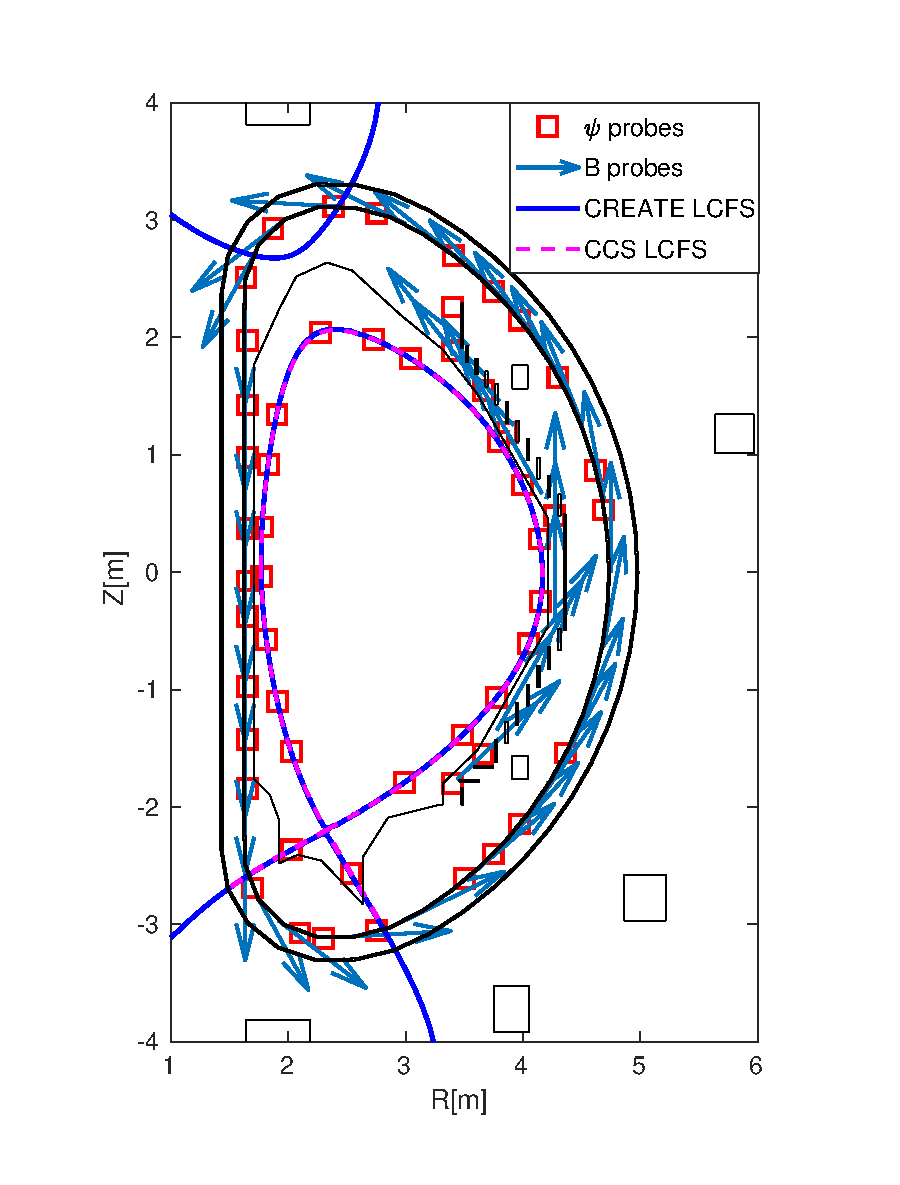
\includegraphics[width=0.6\textwidth]{Chp3/sensors_plots_newDirection.eps}
	\caption{SOF equilibrium reconstructed from CREATE-NL and the CCS code along with the  magnetic field and flux sensors locations.	\label{JT60sensors} }
\end{figure}


\subsection{QST magnetic controller }


The QST magnetic controller  uses the PF coils signals to control the plasma current $I_p$, position and shape, and the FPPC coils signals for plasma position control. The PF coil currents $I_{PF-ref}$ are calculated using an isoflux control approach using proportional-integral(PI) feedback controllers   ~\cite{FBC}. The controller calculates $I_{PF-ref}$ reducing $\delta\Psi_s$ and $\delta\Psi_x$ according to:



\begin{equation}
I_{PF\_ref}(t+\Delta t) = I_{PF}(t_0)+M^\dagger_{PF}\left[G_{SP}\delta\Psi_s(t)+G_{SI}\int_{t_0}^{t}\delta\Psi_s(t)dt+G_{XP}\delta\Psi_X(t)+G_{XI}\int_{t0}^{t}\delta\Psi_x(t)dt\right]~,
\end{equation}

where $\delta\Psi_s$ is the residual between the  LCFS flux and the control point fluxes,   $\delta\Psi_x$ is the difference between the $I_p$ value and its reference, $t_0$ is the initial time , $\Delta t$ is the coil control cycle, $M^\dagger_{PF}$ is the (m $\times$ (n + 1)) control matrix which is the pseudo-inverse of the Green function $M$ calculated using the SVD method; where m is the number of PF coils , n is the number of control points including the evaluated X-point. $G_{SP}$ and $G_{SI}$ are the respective control gains for the PI plasma position and shape feedback controllers, $ G_{XP}$ and $G_{XI}$ are the PI control gains for the $I_p$ feedback control. $G_{SP}$ and $G_{XP}$ are dimensionless and, $G_{SI}$ and  $G_{XI}$ are in $s^{-1}$. \smallskip



The coils voltage command values ($V_{coil-com}$) are calculated considering the mutual interactions between the PF coils an the plasma,the actual values of the PF coil currents, $I_p$ and the mutual inductances. On a real plasma experiment, the  mutual inductances between the plasma and the PF coils are unknown due to the difficulty of measuring them directly. Therefore, they are provided by the CCS method. The controller calculates command values of PF coils voltages according to the following equation:



\begin{equation}
V_{com}=G_{vt}\left[M_{coil}\frac{(I_{coil\_ref}-I_{coil\_meas})}{dt}+ \frac{M_{plasma\_now} \cdot I_{p\_now} - M_{plasma\_ bfr} \cdot I_{p\_bfr}}{dt}\right]~,
\end{equation}

where $M_{coil} $ represents the mutual inductances between the coils, $I_{coil\_meas}  $ are the measured coil currents,  $M_{plasma\_now}$ and $ M_{plasma\_ bfr}$ are the mutual inductances between the plasma and the coils at the current and previous time step,$  I_{p\_now} $  and  $ I_{p\_bfr} $ are the measured plasma current at the current and previous time step  and $ G_{vt} $ is the voltage transformer gain.
\smallskip

On the other hand,the in-vessel FPPC coils currents $ (I_{FPPC\_ref})  $ are calculated with an isoflux control approach which uses proportional-differential (PD) feedback control. In order to reduce  the residual between the LCFS flux and two specified control points ( $ \Psi_{SF} $)  the controller calculates  $ (I_{FPPC\_ref})  $ using:

\begin{equation}
I_{FPPC\_ref}(t+\Delta t)=I_{FPPC}(t_0)+ M^\dagger_{FPPC}\left[G_{FP}\delta \Psi_{SF}(t) + G_{FD}\frac{d}{dt}\delta\Psi_{SF}(t) \right] ~,
\end{equation}

where $ M^\dagger_{FPPC}$ is the $ 2 \times 2$ control matrix which is the pseudo-inverse of the Green function $M_{FPPC}$, $ G_{FP} $ and $ G_{FD} $
are the respective PD feedback gains for the plasma position control. $ G_{FP} $ is dimensionless and $ G_{FD} $ is in $s$.



\section{Simulation results}	

 The simulations for  the JT60-SA CREATE-NL model ,the XSC, the CCS reconstruction method and the QST controller  were programmed on top of  \textsc{Matlab} and \textsc{Simulink} blocks. This  section will address in detail the outcome of the control simulations using a linearized equilibrium given by CREATE-NL for JT60-SA, Scenario~2 at the SOF time frame. The first results to be presented correspond to a  gap-based controller  using the XSC with different tests cases.
 \smallskip
 
 
 The second part of the results corresponds to isoflux controllers using the XSC  with a LCFS reconstruction given by CREATE and also given by the CCS method, as well as the QST controller with the LCFS reconstructed by the CCS method and by CREATE. The figures ~\ref{JT60controlscheme} and ~\ref{JT60FBCcheme} show an overall control block scheme for the simulations.   Figure ~\ref{JT60controlscheme} corresponds to a configuration using the XSC where the LCFS can be obtained through the CCS method or from the CREATE model. It is worth to point out the existence of the block localized on the bottom part of the scheme called "Vertical Stability Control" along with the XSC. The task of this block is to vertically stabilize the plasma by exploiting the in-vessel coils, which are able to guarantee a faster response due to the fact that the magnetic field generated does not have to penetrate the vessel structures  ~\cite{NCruz}. This controller calculates the voltages at the FPPC coils with the equation:
 
 \begin{equation}
 V_{FPPC}(t)=k_1I_{FPPC}(t)+ k_2\dot{z}_p(t)
 \label{FPPC_eqs}
 \end{equation}   
 
 By tuning the gains $k_1$ and $k_2$ from equation ~\ref{FPPC_eqs} is possible to obtain zero velocity in the vertical plasma direction while maintaining low imbalance current$  I_{FPPC} $ in the in-vessel coils~\cite[Sec.~4.1]{NCruz}.  In addition should also be notice the block "Ip Control" which is a Plasma current Controller, which tracks the desired value of the plasma current ~\cite{de2014shape}.

 
 
\begin{figure}
	\centering
	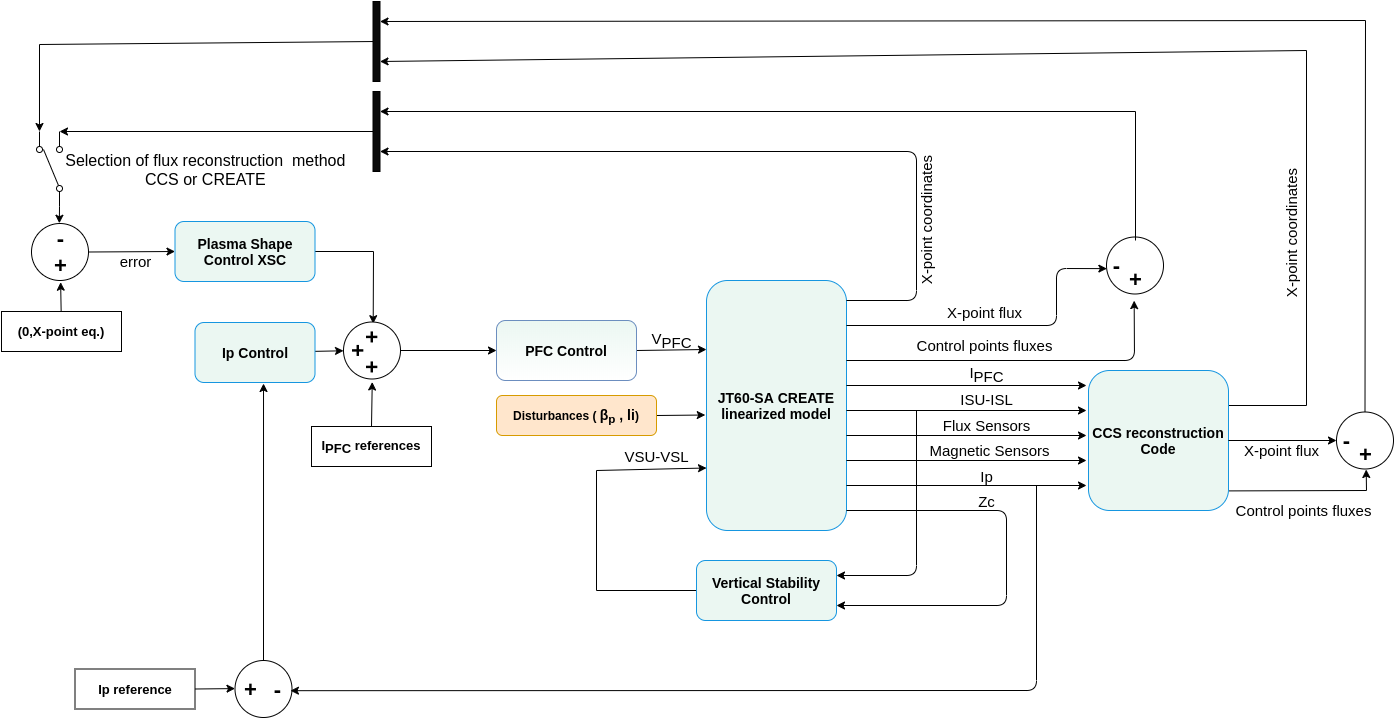
\includegraphics[width=1.05\textwidth]{Chp3/JT60Schemes1.png}
	\caption{	\label{JT60controlscheme}JT-60SA overall control scheme with the CREATE linearized model and the CCS LCFS reconstruction method  using the XSC for an isoflux control approach.}
\end{figure}

Figure ~\ref{JT60FBCcheme} depicts a configuration using the QST controller reciving as inputs the magnetic fluxes measured at the control points reconstructed either by the CCS method or by the CREATE linearized model.
\smallskip
 
\begin{figure}
	\centering
	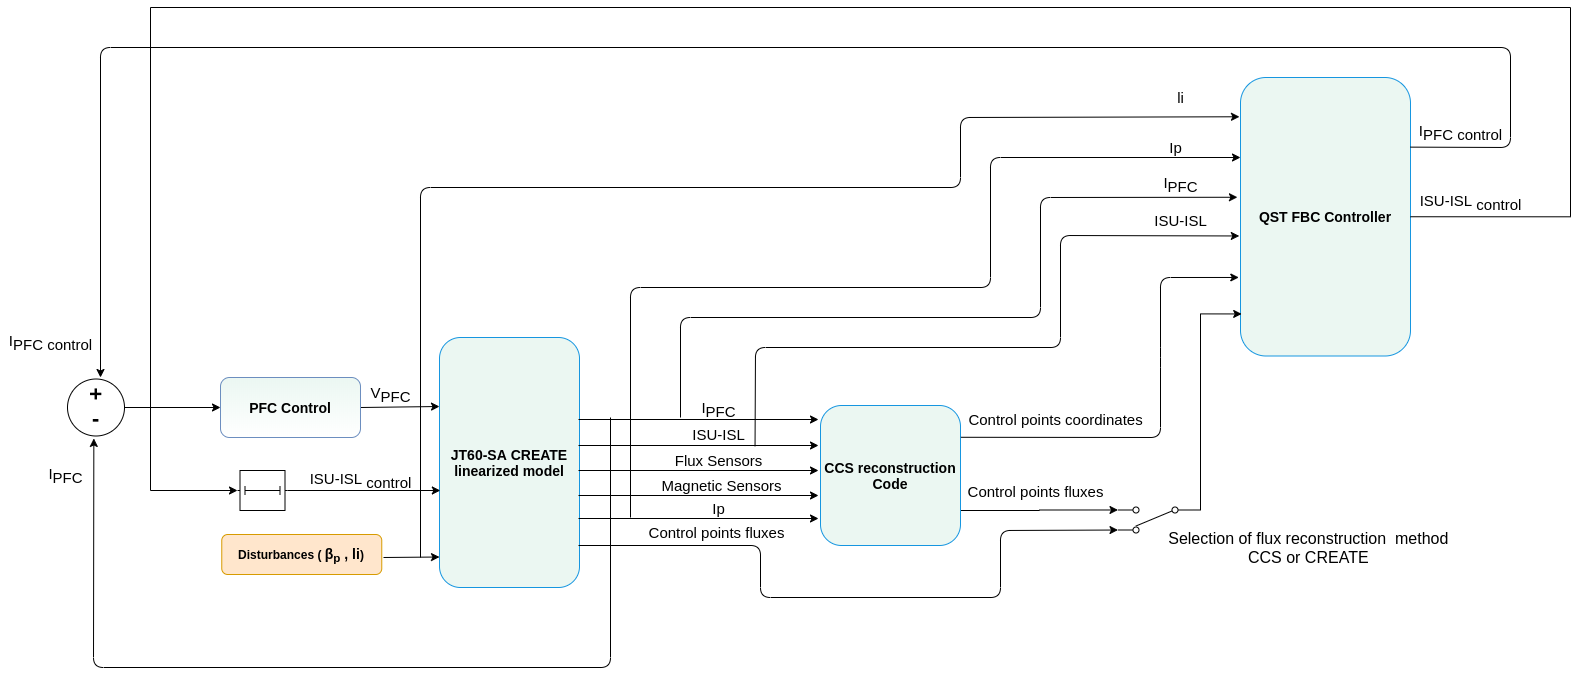
\includegraphics[width=1.05\textwidth]{Chp3/JT60SchemeFBCnew.png}
	\caption{	\label{JT60FBCcheme} Isoflux control JT-60SA overall scheme with  a block for the  CREATE JT60-SA linearized model, a block for reconstructing  the magnetic fluxes with the CCS method and the QST controller. }
\end{figure}



\subsection{Disturbances}


As far as plasma magnetic control is concerned, the JT60-SA linearized model disturbances have been modeled as variations of $\beta_p$ and $l_i$. This disturbances should be in principle rejected by the control systems and maintain in the most accurate possible way the plasma equilibrium.  The following set of disturbances have been considered: 

\begin{itemize}
	\item \textbf{Disturbance \#1} refers to the behavior of~$\beta_p$ and~$l_i$ soon after the current flattop is reached, as it was modeled in~\cite{urano2015development} (in this paper we assume that the flattop is reached at~$t\sim 20$~s). As an example, the correspondent time traces are shown in figure~\ref{Urano}\footnote{The time behavior of both~$\beta_p$ and~$l_i$ have been estimated starting from the spatial profiles for both plasma density and temperature envisaged for Scenario 2.}.
	
	


%	\item \textbf{Disturbance \#2} refers to the behaviour of ~$\beta_p$  due to the presence of an Edge-Localized Mode~(ELM). As described in~\cite[p.~34]{JT60SA:PID}, during the flattop an instantaneous drop in~$\beta_p$ of ~$0.05~\beta_{p_{eq}}$ is followed by and exponential recovery with a time constant of~0.05~s with a frequency 10~Hz. Note that for this disturbance~$l_i$ does not change.% remains as~$l_{i_{eq}}$, these behaviors are shown in Fig.~\ref{figure:ELM}.
	
	\item \textbf{Disturbance \#2} refers to the behaviour of~$\beta_p$ and~$l_i$ when a compound ELM\footnote{A compound ELM is commonly referred as multiple clearly distinguishable
	crash events causing large energy losses \cite{Meyer2017}.} appears during the flattop.  As described in~\cite[p.~34]{JT60SA:PID}, an instantaneous drop   in~$\beta_p$ of ~$0.05~\beta_{p_{eq}}$ is followed by and exponential recovery with a time constant of~0.05~s with a frequency 10~Hz, $l_i$ is described by an instantaneous drop of~$0.06~(l_{i_{eq}}-0.5)$ followed by and exponential recovery with a time constant of 0.05~s with a frequency 10~Hz. The time traces for~$\beta_p$ and~$l_i$ are described in figure~\ref{cmpELM}.
	


	
	\item \textbf{Disturbance \#3} describes an instantaneous drop in~$l_i$ of~$0.2~(l_{i_{eq}}-0.5)$ without recovery, simultaneous with a drop on~$\beta_p$ of~$0.2~\beta_{p_{eq}}$ followed by a recovery exponential time of~1~s~\cite[p.~34]{JT60SA:PID}, which are typical of a so called \emph{Minor disruption}. The correspondent time traces for both~$\beta_p$ and~$l_i$ are reported in figure~\ref{MnrDisrp}.
\end{itemize}


	\begin{figure}[h]
	\centering
	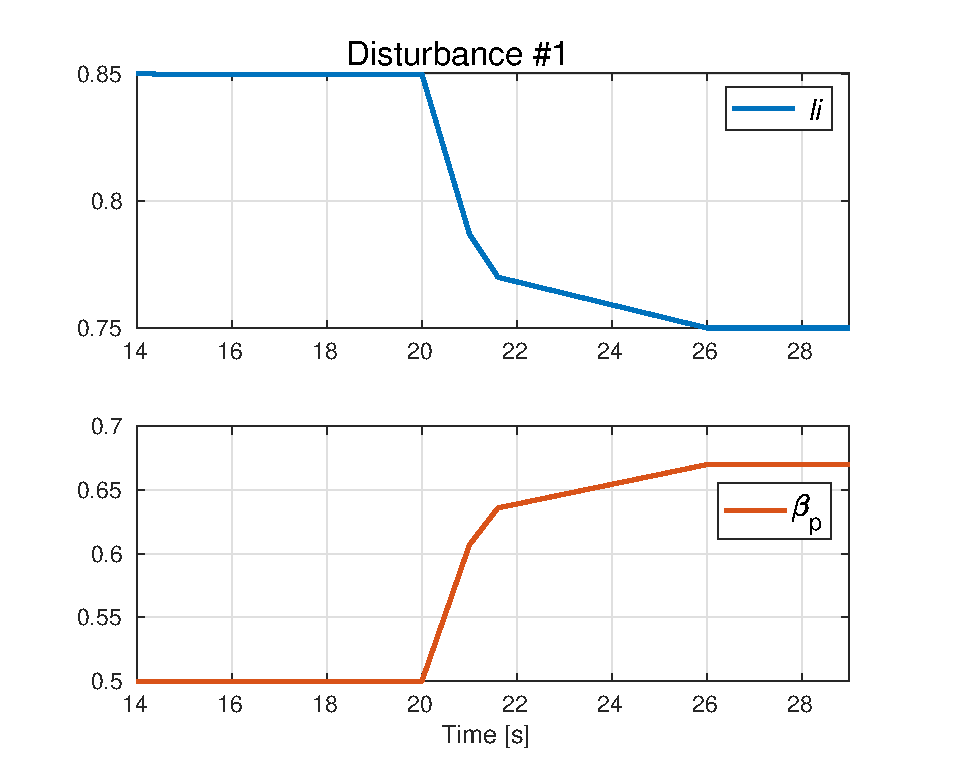
\includegraphics[width=0.5\textwidth]{Chp3/Dist_1_Urano.eps}
	\caption{Poloidal beta and internal inductance time traces for Disturbance~\#1 that models the expected disturbance soon after the plasma current flattop is reached (at~$t\sim 20 $~s), according to what has been considered in~\cite{urano2015development}.	\label{Urano} }
\end{figure}

	\begin{figure}[h]
	\centering
	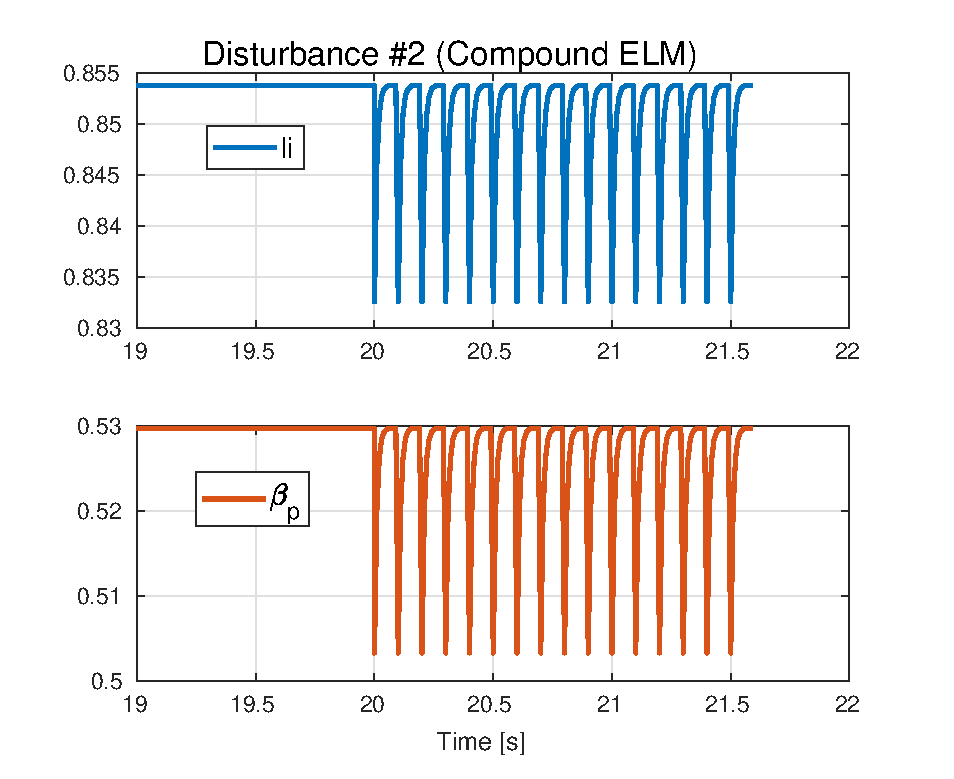
\includegraphics[width=0.5\textwidth]{Chp3/Dist_2_cmp_ELM.eps}
	\caption{Poloidal beta and internal inductance time traces for Disturbance~\#2 that models the behavior of these variables due to the presence of a compound ELM as defined in~\cite{JT60SA:PID}.	\label{cmpELM} }
\end{figure}


\begin{figure}[h]
	\centering
	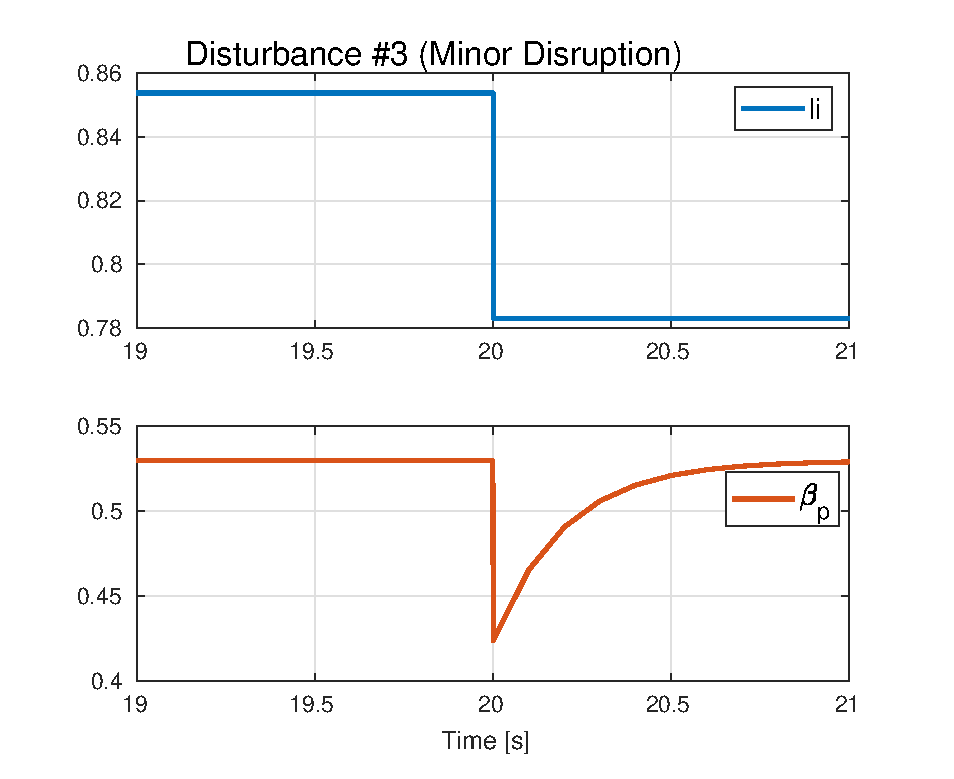
\includegraphics[width=0.5\textwidth]{Chp3/Dist_3_minor.eps}
	\caption{Poloidal beta and internal inductance time traces for Disturbance~\#3 that models the behavior of these variables due to the presence of a Minor disruption as defined in~\cite{JT60SA:PID}.	\label{MnrDisrp} }
\end{figure}



\subsection{Gap-based XSC}

JT-60SA represents a relevant benchmark to further validate the gap-based control approach, given the high beta regimes that are envisaged during its operation, which represent a challenge from the plasma magnetic control perspective. Different test cases are considered to assess the performance of the proposed shape controller, with the aim of defining an optimal set of gaps to be controlled. This sections evaluates the steady-state performance of the plasma shape controller under different choices for \emph{gaps} to be controlled. \smallskip

 All around the first wall an equally spaced distribution of~85 gaps was considered as shown in figure~\ref{figure:85_gaps}. It should be noticed that all different selections of controlled gaps considered in this paper include the two vertical gaps in the divertor zone, which allows to control the strike-points, and hence the position of the X-point. Other than the whole set of~85 gaps,  three additional choices are considered. The first one is reported in figure ~\ref{figure:20_gaps}, which consists of~20 gaps equally spaced along the first wall. Moreover, the selection of~8 and~6 gaps that correspond with the control segments considered by the isoflux controllers presented in~\cite{miyata2013study} and~\cite{Miyata:2014}, respectively, have been also considered (see  figures ~\ref{figure:8_gaps} and~\ref{figure:6_gaps}). These two latter options are the outcome of preliminary studies aimed at controlling the plasma shape with a set of almost decoupled loops, i.e.  SISO, while the XSC approach proposed in this section is intrinsically MIMO. Moreover, it is worth to remark that, although in~\cite{miyata2013study} and~\cite{Miyata:2014} the 8 and 6 gap options have been used with an isoflux control approach, here the same control segments have been used to design the XSC adopting a gap-based approach.\smallskip


\begin{figure}[h]
	\centering
	\begin{subfigure}[b]{0.32\textwidth}
		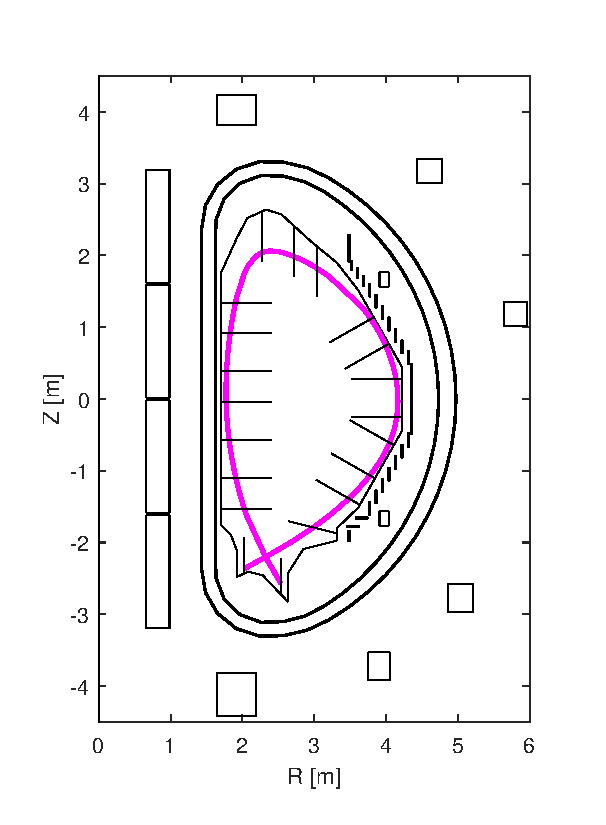
\includegraphics[width=\textwidth] {Chp3/20_gaps.eps}  
		\caption{The~20 gaps used to assess the performance of plasma shape controller.	\label{figure:20_gaps} }
	\end{subfigure}
	~
	\begin{subfigure}[b]{0.32\textwidth}
		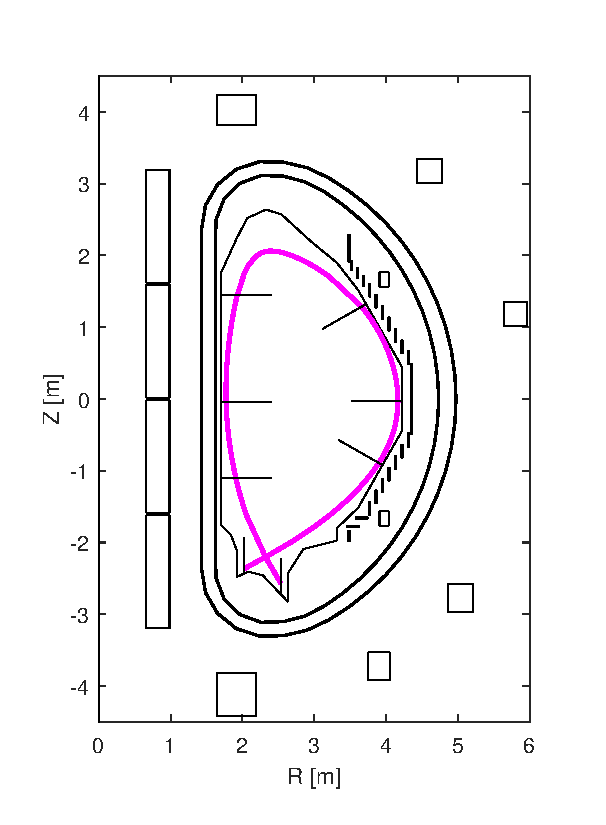
\includegraphics[width=\textwidth]{Chp3/8_gaps.eps} 
		\caption{The~8 control segments by the isoflux controller proposed in~\cite{miyata2013study}.\label{figure:8_gaps}}
	\end{subfigure}
	~
	\begin{subfigure}[b]{0.32\textwidth}
		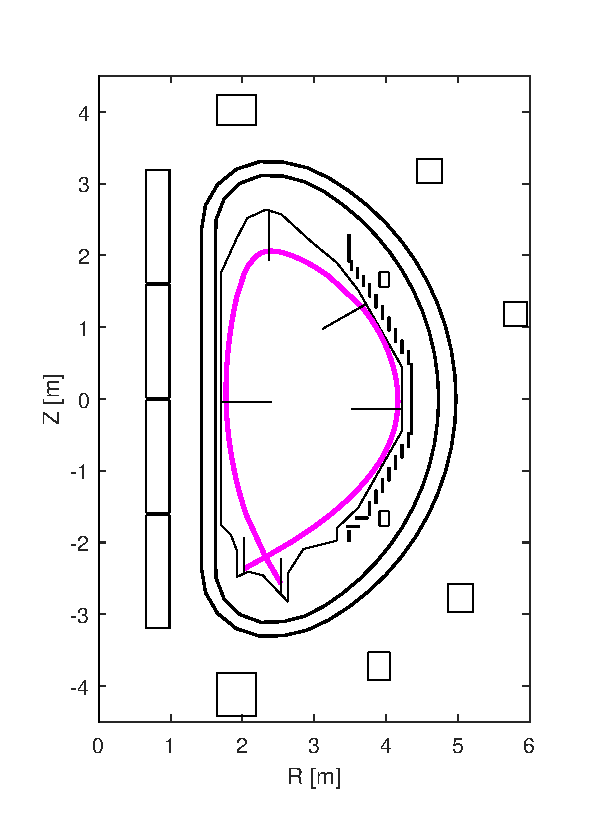
\includegraphics[width=\textwidth]{Chp3/6_gaps.eps} 
		\caption{ The~6 control segments used by the isoflux controller proposed in~\cite{Miyata:2014}. \label{figure:6_gaps}}
	\end{subfigure}
	
\caption{Different choices for the set of controlled gaps used for gap controller.} \label{figure:gapChoices}
\end{figure}


The comparison between the various considered gap sets for the different disturbances test cases is summarized in Table~\ref{gapTable}. This table shows the \emph{root-mean-square error}~(RMSE) between the reference shape and the shape obtained at steady-state after the occurrence of the disturbances. For all the cases reported in Table~\ref{gapTable}, the RMSE has been computed on the set of~85 gaps shown in figure~\ref{figure:85_gaps}, even when not all of them are controlled. \smallskip

\begin{table}[h]
	\centering
	\begin{tabular}{|l|c|c|c|c|}
		\hline
		\rowcolor{color2}
		\multicolumn{5}{|c|}{\textbf{Steady-state RMSE  mm}}                        \\ \hline
		\rowcolor{color1}
		\multicolumn{1}{|c|}{}              & 85 gaps & 20 gaps & 8 gaps  & 6 gaps  \\ \hline
		Disturbance \#1                     & 7.7     & 8.7     & 31.2    & 19.8    \\ \hline
		Disturbance \# 2 (compound ELM)      & $\sim 0$ & $\sim 0$ & $\sim 0$ & $\sim 0$ \\ \hline
		Disturbance \# 3 (Minor disruption) & 6.1     & 7.8     & 26.9    & 16.3    \\ \hline
	\end{tabular}
	\caption{Steady-state RMSE values for the different choices of number of controlled gaps and for the different disturbances test cases. }
	\label{gapTable}
\end{table}


It turns out that, according to this preliminary analysis, the rejection of the disturbances induced by the compound ELMs at steady-state is not an issue at JT-60SA, whatever is the set of gaps that is controlled. Indeed, figure~\ref{figure:RMSE_ELM} shows the~RMSE time traces for Disturbance~\#2 (compound ELMs), being the RMSE computed on the set of~85 gaps shown in figure ~\ref{figure:85_gaps} for all the considered options. It turns out that, whatever gap set is used, the controller has almost the same behavior, with a slightly worse performance of the~6 and~8 gap options. Being a periodic disturbance, the compound ELMs have been applied only during the first part of the simulation, in order to evaluate the steady-state performance of the controller. However, from figure ~\ref{figure:RMSE_ELM} it can be noticed that the rejection of the compound ELMs is not a concern even during the transients, being the maximum RMSE~$\sim 2$ mm. \smallskip

\begin{figure}[!thb]
	\begin{center}
		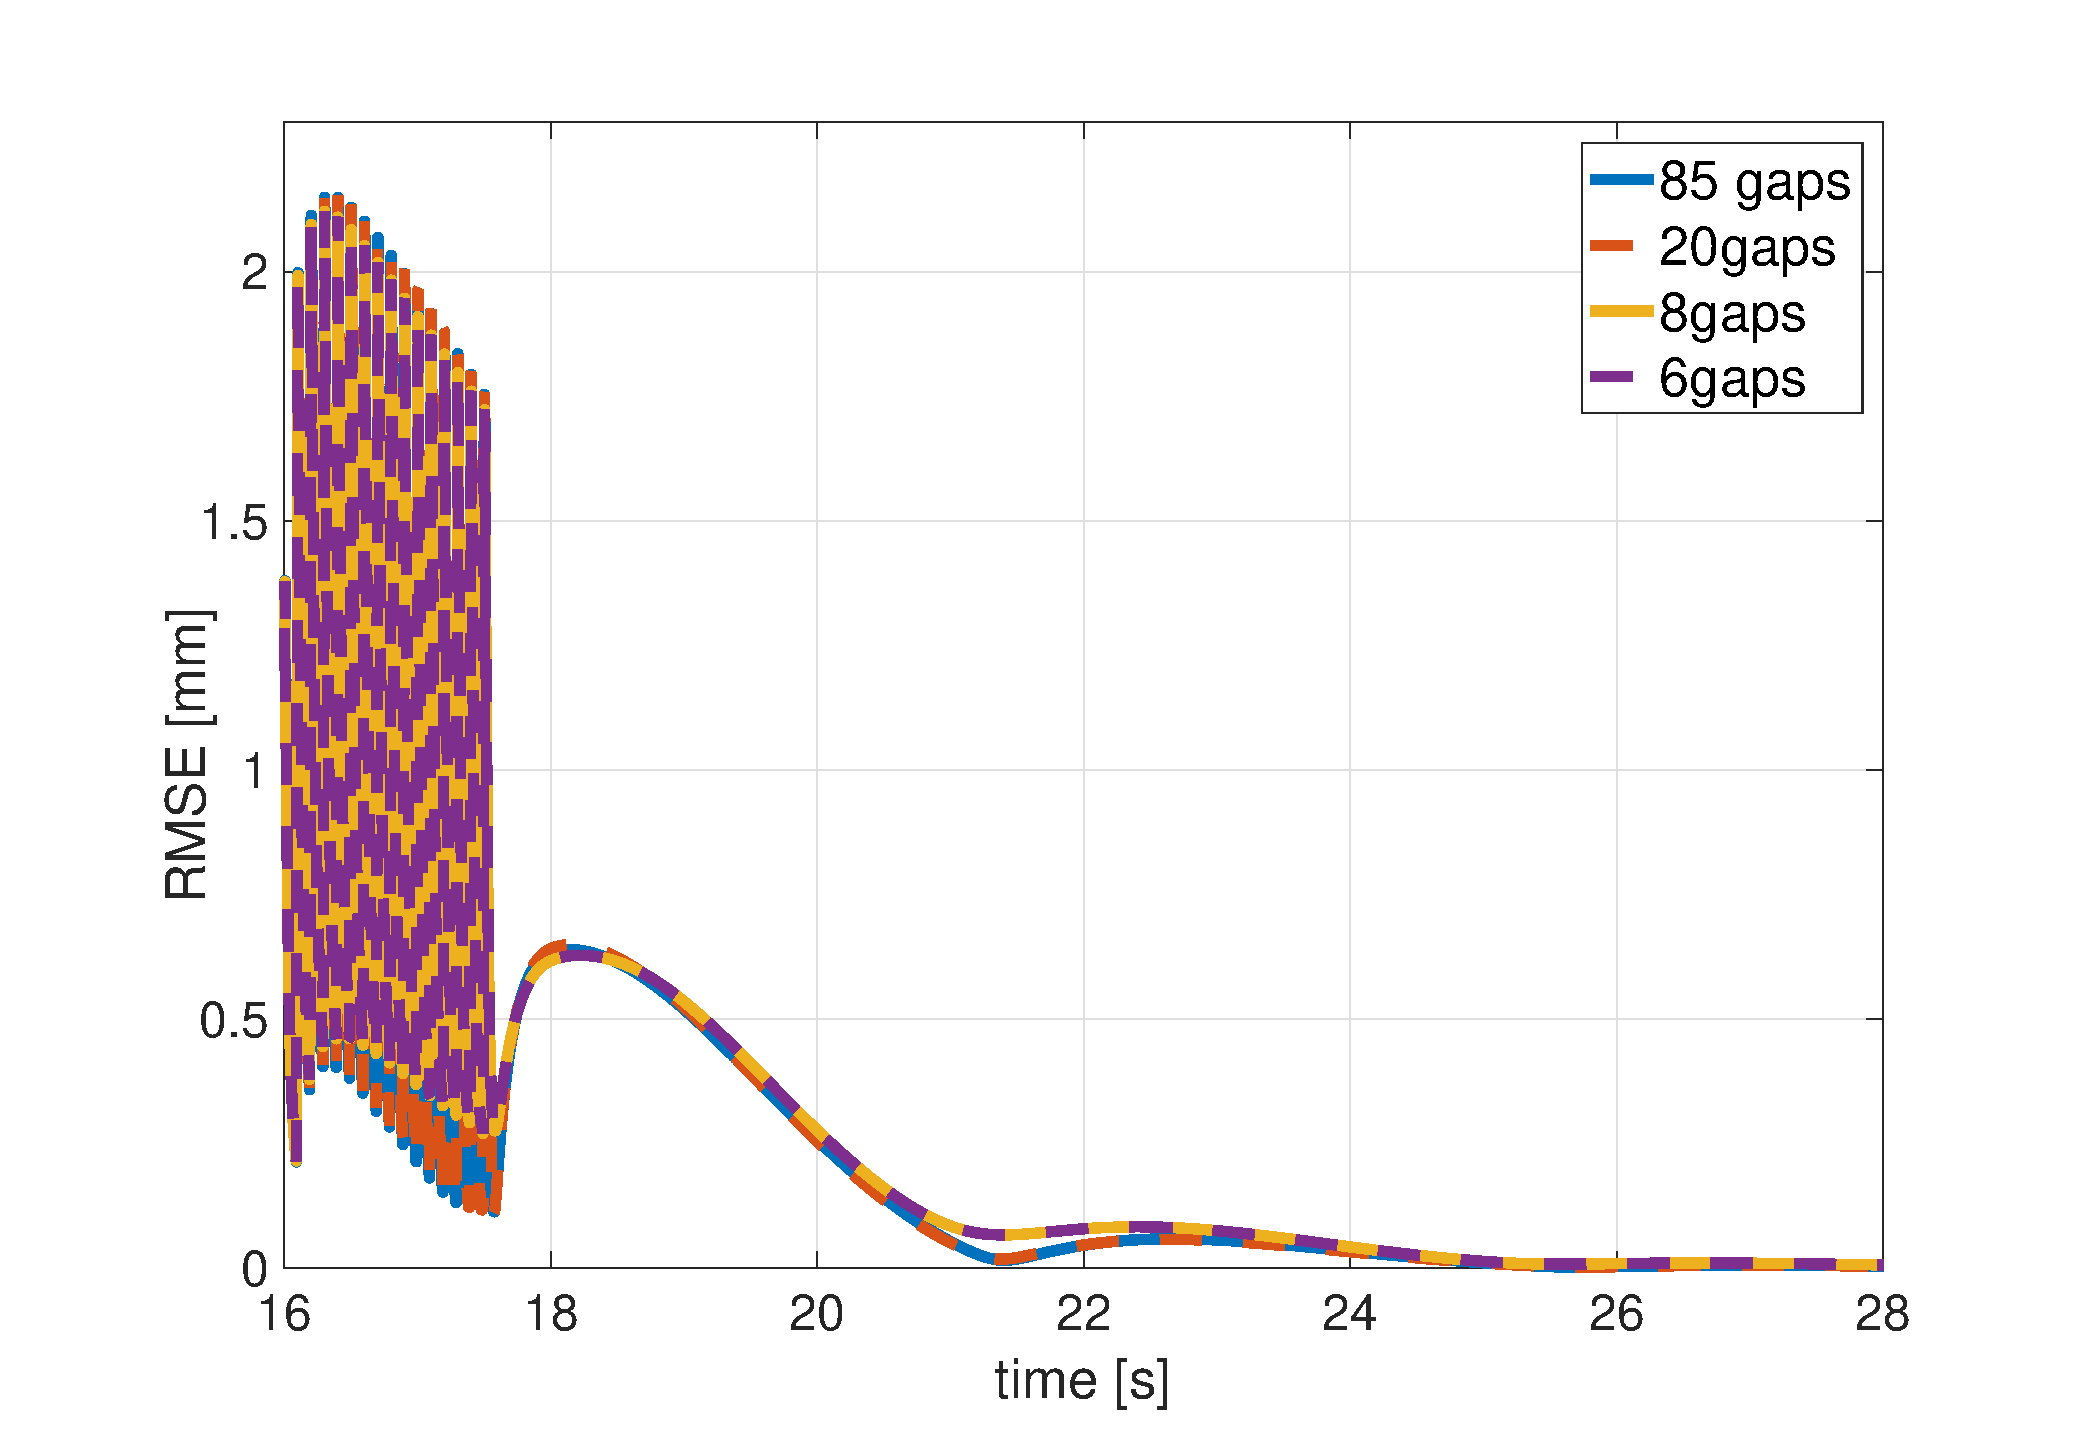
\includegraphics[width=8.5cm]{Chp3/RMSE_ELM.eps}
	\end{center}\caption{RMSE time traces for the different gaps selections in the presence of Disturbance~\#2 (compound ELMs). For all the considered cases, the RMSE is computed on the set of~85 gaps shown in figure ~\ref{figure:85_gaps}.}\label{figure:RMSE_ELM}
\end{figure}




For the other two considered cases, at steady-state, the selection of~85 and~20 gaps have a considerable better~RMSE in comparison with the selection of~8 and~6 gaps. As outlined in Table~\ref{gapTable}, the worst case corresponds to the selection of~8 gaps with the presence of Disturbance~\#3 (Minor disruption) during the flattop. As an example, figure~\ref{figure:minor} shows a comparison of the steady-state shape obtained for the~8 and~20 gaps options when the Minor disruption in considered. Figure~\ref{figure:RMSE} shows the~RMSE time traces for this disturbance and it can be noticed that the~20 gaps option gives better results with respect to the~8 and~6 gaps cases also during the transient, and not just in steady-state.  In particular, in the~6 and~8 gaps cases, being the number of controlled gaps less than the number of the actuators available for plasma shape control, the steady-state error on the controlled gaps is practically zero. However, not being these two sets of gaps \emph{well representative} of the whole plasma boundary, minimizing the error on such sets does not minimize the error on the whole boundary, as shown in figure~\ref{figure:RMSE}.\smallskip

\begin{figure}[!thb]
	\begin{center}
		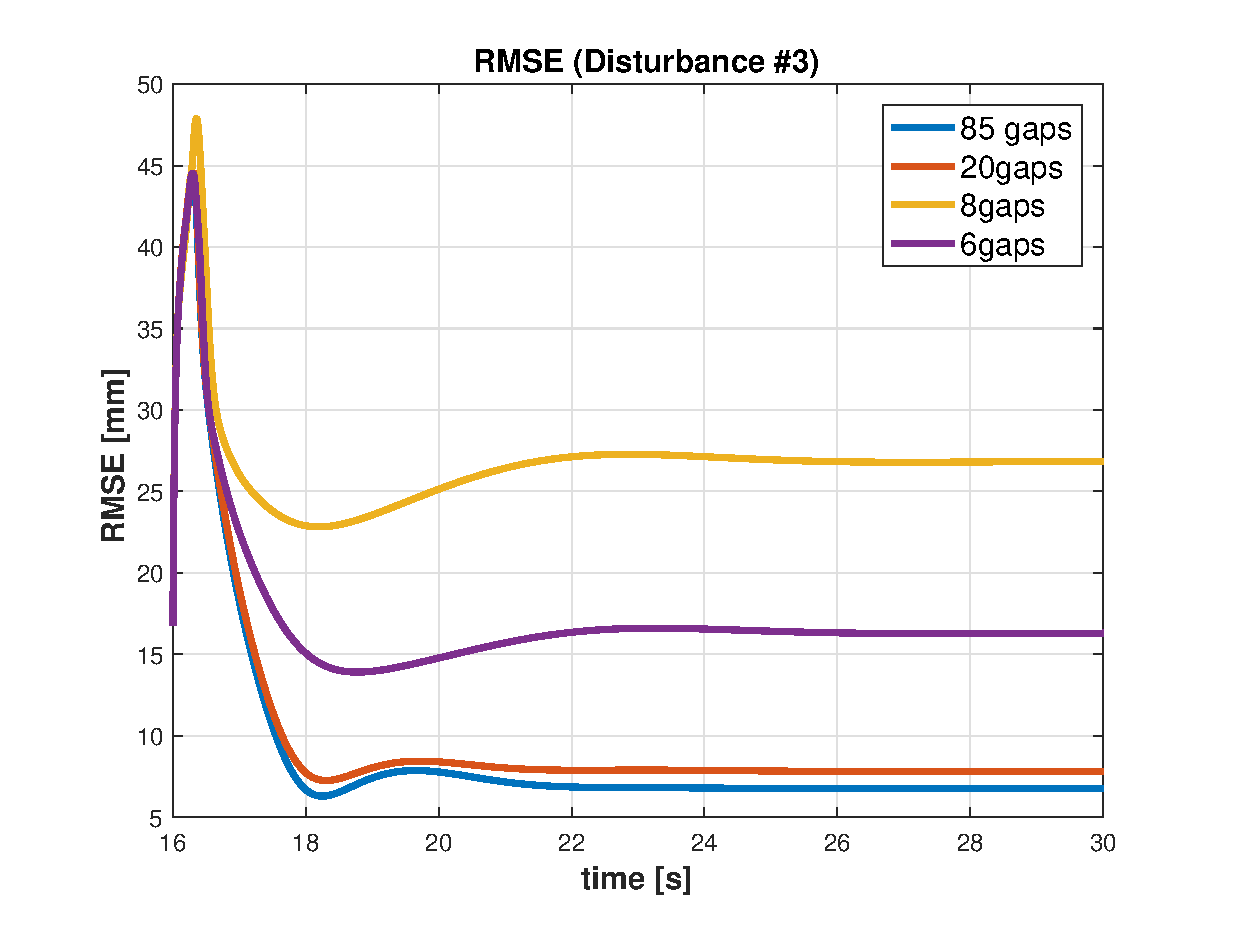
\includegraphics[width=8.5cm]{Chp3/RMSE_minor.eps}
	\end{center}\caption{RMSE time traces for the different gaps selections in the presence of Disturbance~\#3 (Minor disruption). For all the considered cases, the RMSE is computed on the set of~85 gaps shown in Fig.~\ref{figure:85_gaps}.}\label{figure:RMSE}
\end{figure}

It should be also noticed that the~6 gaps option considered in~\cite{Miyata:2014} gives better performance than the set of~8 gaps chosen in~\cite{miyata2013study}. Indeed, with the latter set, there is a worse control of the plasma top region, as shown in figure ~\ref{figure:minor_top}. Moreover, for the two options with~85 and~20 equally spaced gaps there is no practical difference between the reference shape and the one attained at steady-state. The fact that there is no practical improvement in controlling 85 gaps rather than 20, can be better understood recalling that~$\bar{n}<n_{PF}$ singular values are used to compute the control matrix as the pseudo-inverse~$C^\dag$ in~\eqref{equation:XSC_new}. In particular, only the singular values that are greater than the~5\% of the greatest one are used to compute~$C^\dag$. \smallskip


\begin{figure}[h]
	\centering
	\begin{subfigure}[b]{0.32\textwidth}
		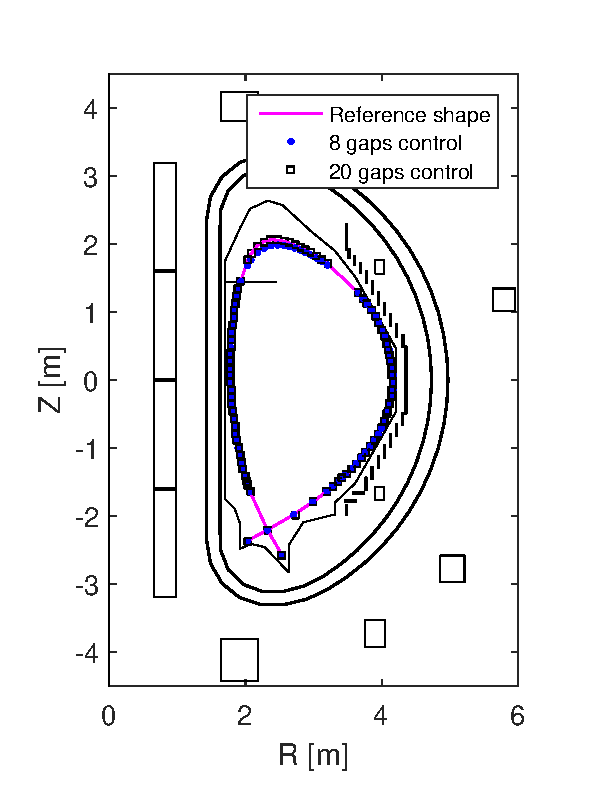
\includegraphics[width=\textwidth] {Chp3/Ref_20gaps_8gaps_minor_2.eps}  
		\caption{Poloidal cross-section of JT-60SA.\label{figure:minor_big} }
	\end{subfigure}
	~
	%	~ %add desired spacing between images, e. g. ~, \quad, \qquad, \hfill etc. 
	%(or a blank line to force the subfigure onto a new line)
	\begin{subfigure}[b]{0.32\textwidth}
		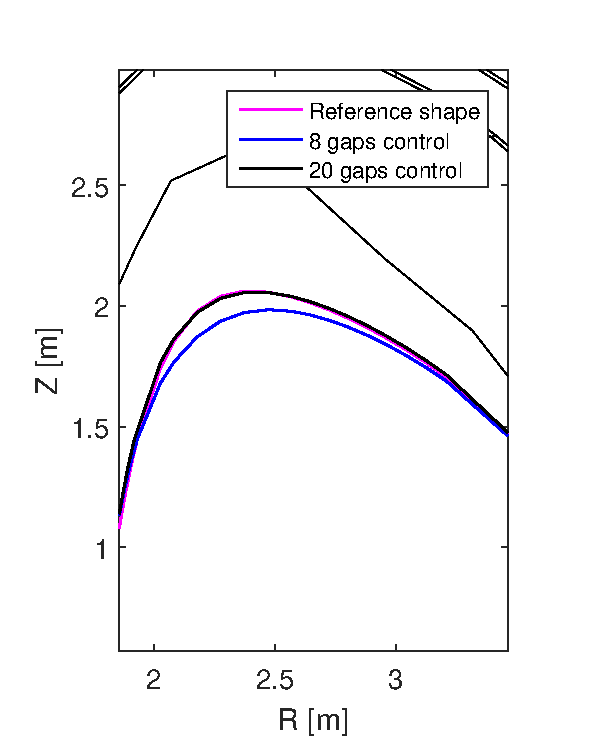
\includegraphics[width=\textwidth]{Chp3/zoom_Ref_20gaps_8gaps_minor_top_2.eps} 
		\caption{Detailed view of the plasma top region.\label{figure:minor_top}}
	\end{subfigure}
	~
	\begin{subfigure}[b]{0.32\textwidth}
		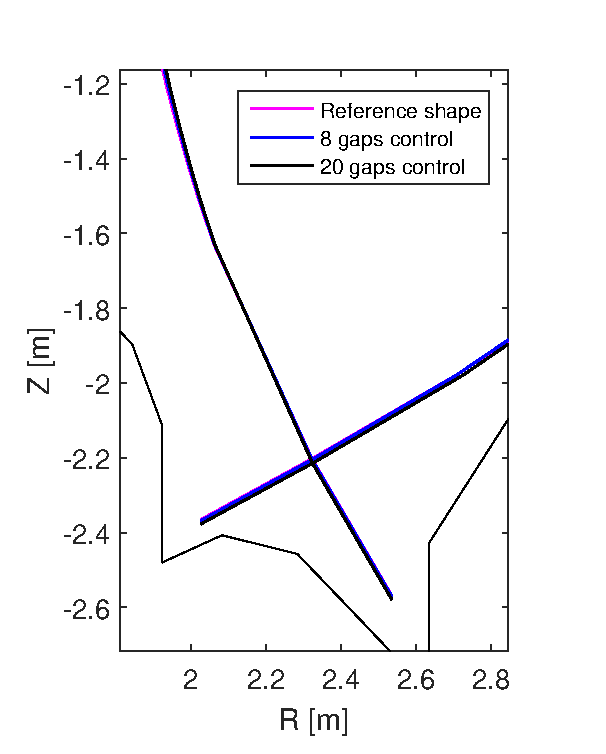
\includegraphics[width=\textwidth]{Chp3/zoom_Ref_20gaps_8gaps_minor_strike_2.eps} 
		\caption{Detailed view of the plasma divertor region. \label{figure:minor_strike}}
	\end{subfigure}
	
	
	\caption{ Comparison of the shape controller performance in the presence of Disturbance~\#3 (Minor disruption). The two cases of 8 and 20 gaps are considered.}
	\label{figure:minor}
\end{figure}








\subsection{Isoflux XSC and QST controller }

As mentioned in the previous section, simulations with an isoflux control approach using the CREATE linearized model and the XSC along with the QST reconstruction and control tools were carried out. The same three disturbances (see figure~\ref{Urano},~\ref{cmpELM} and ~\ref{MnrDisrp}) and JT60-SA equilibrium scenario from the simulations in last section were used for these test cases for a different number of control points.  Due to the vast extension of results, this section will focus on analyze the case for 8 control points in the presence of a Minor disruption with the XSC and the QST controller. Figure~\ref{all_points} shows the control points configurations used for carrying out the simulations with an isoflux shape controller as well as the LCFS's reconstructed by CREATE and  the CCS method at steady-state in the presence of a Minor disruption(Disturbance~ $\#3$). 
\smallskip

For the control and reconstruction points configurations a selection of 19 equally spaced descriptors was used (see figure~\ref{19gaps_isoflux}),  along with the previous 8 and 6 points configurations used for the gap controller. As mentioned before, the CCS method allows a maximum of 19 points for the fluxes reconstruction and the QST controller a maximum of 10 control points,due to these  limitations the 19 segments scenario is only  feasible using the XSC.
\smallskip


\begin{figure}[h]
	\centering
	\begin{subfigure}[b]{0.32\textwidth}
		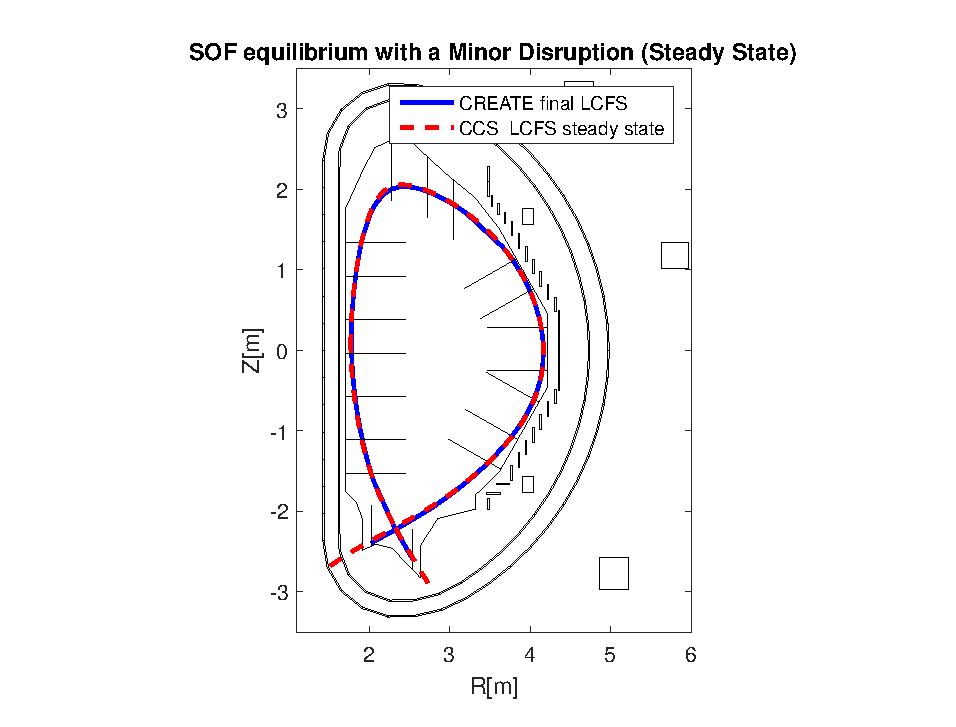
\includegraphics[trim={2.3cm 0 2.3cm 0},clip,height=5.75cm] {Chp3/19_gaps_mnr_disrp_SS_comp.eps}  
		\caption{The~19 control segments used to assess the performance of plasma shape controller.\label{19gaps_isoflux} }
	\end{subfigure}
	~
	%	~ %add desired spacing between images, e. g. ~, \quad, \qquad, \hfill etc. 
	%(or a blank line to force the subfigure onto a new line)
	\begin{subfigure}[b]{0.32\textwidth}
		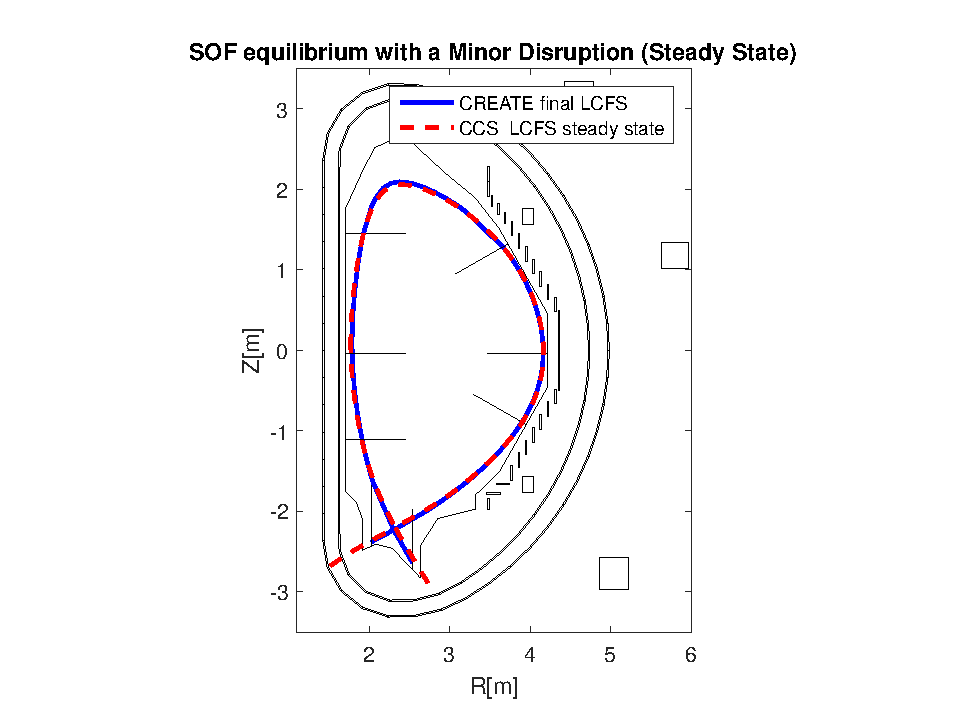
\includegraphics[trim={2.3cm 0 2.3cm 0},clip,height=5.75cm]{Chp3/8_gaps_mnr_disrp_SS_comp.eps} 
		\caption{  The~8 control segments by the isoflux controller proposed in~\cite{miyata2013study}. \label{8gaps_isoflux}}
	\end{subfigure}
	~
	\begin{subfigure}[b]{0.32\textwidth}
		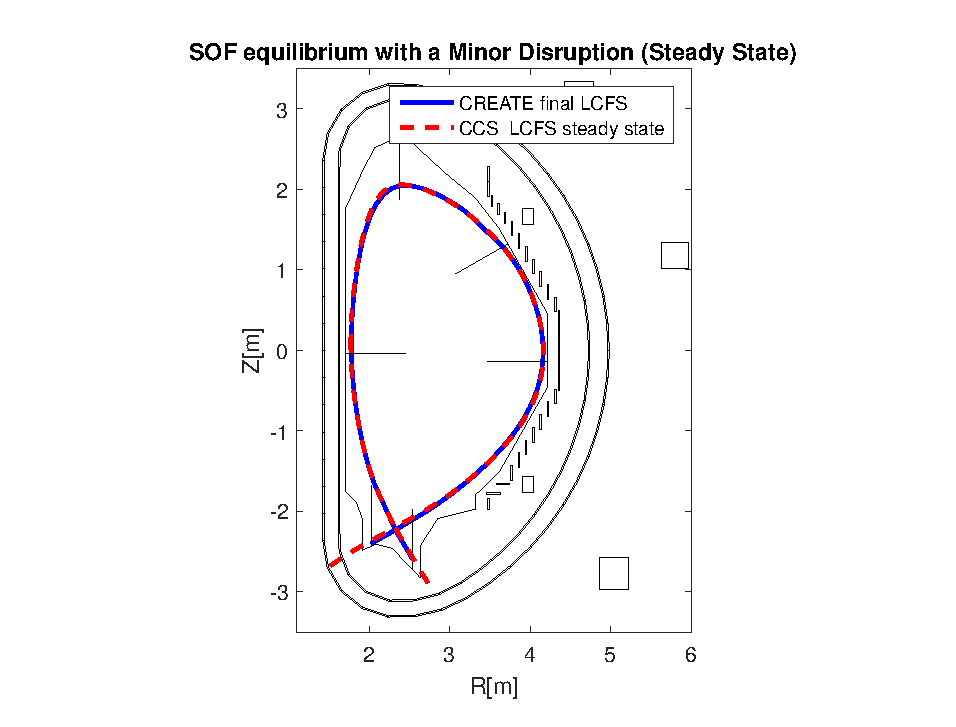
\includegraphics [trim={2.3cm 0 2.3cm 0},clip,height=5.75cm]  {Chp3/6_gaps_mnr_disrp_SS_comp.eps} 
		\caption{  The~6 control segments used by the isoflux controller proposed in~\cite{Miyata:2014}.    \label{6gaps_isoflux}}
	\end{subfigure}

\caption{LCFS reconstructed by CREATE and the CCS code  for the JT60-SA scenario~2 SOF equilibrium with a Minor disruption at steady-state for the three considered selection of control segments using the XSC with an isoflux approach.}\label{all_points}

\end{figure}

Figure~\ref{compFBC_XSC_ss} compares the steady-state LCFS's for the same disturbance and equilibrium using both controllers, at first glance it is not possible to identify any visible difference between the two controllers, which allows a first conclusion that both controls reject the disturbance and maintain the reference plasma shape in steady-state. For further study in figures ~\ref{XSC_20s} and  ~\ref{FBC_20s} is presented the behavior of both controllers at the time instant where their fluxes errors are on their highest value, this happens around 2 ms for the case of the XSC and 65 $\mu$s for the QST control after the Minor disruption takes place. From these figures is possible to  observe that there is a noticeable plasma shape difference in comparison with the one from the equilibrium, specially   on the radial outer region and secondly is visible that the difference between the equilibrium and the steady-sate shape  is smaller for the QST controller case.     
\smallskip

\begin{figure}[h]
	\centering
		\begin{subfigure}[b]{0.32\textwidth}
		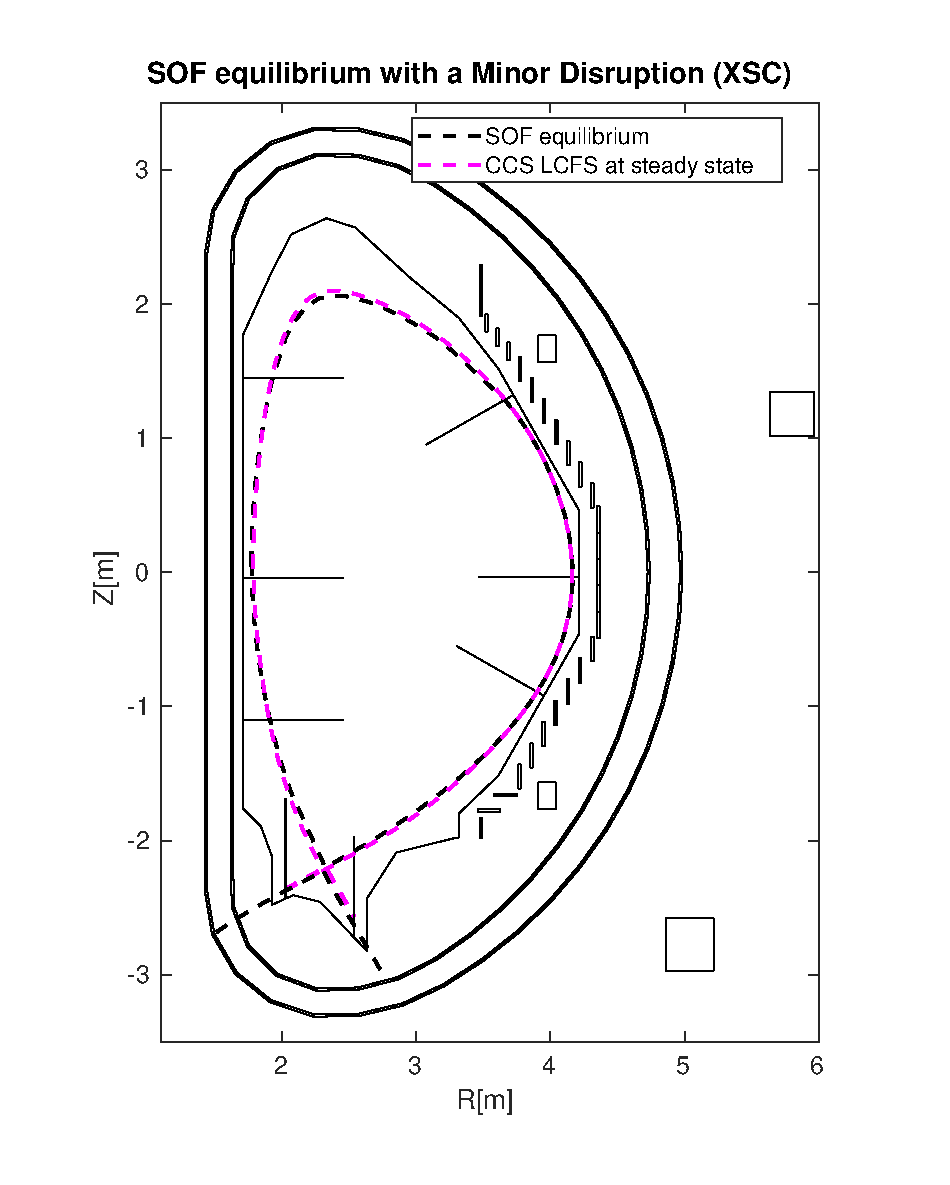
\includegraphics[height=8.75cm] {Chp3/Results_iso/8_gaps_mnr_disrp_equilVsLCFS.eps}  
		\caption{Comparison between the reference shape (i.e., the shape at the considered equilibrium) and the LCFS reconstructed by the  CCS code at steady-state in the presence of the Minor disruption  using the XSC for the plasma shape, when 8 control segments are considered.
		\label{XSC_isoflux_ss} }
			\end{subfigure}
	\hspace{2 cm}
				\begin{subfigure}[b]{0.32\textwidth}
			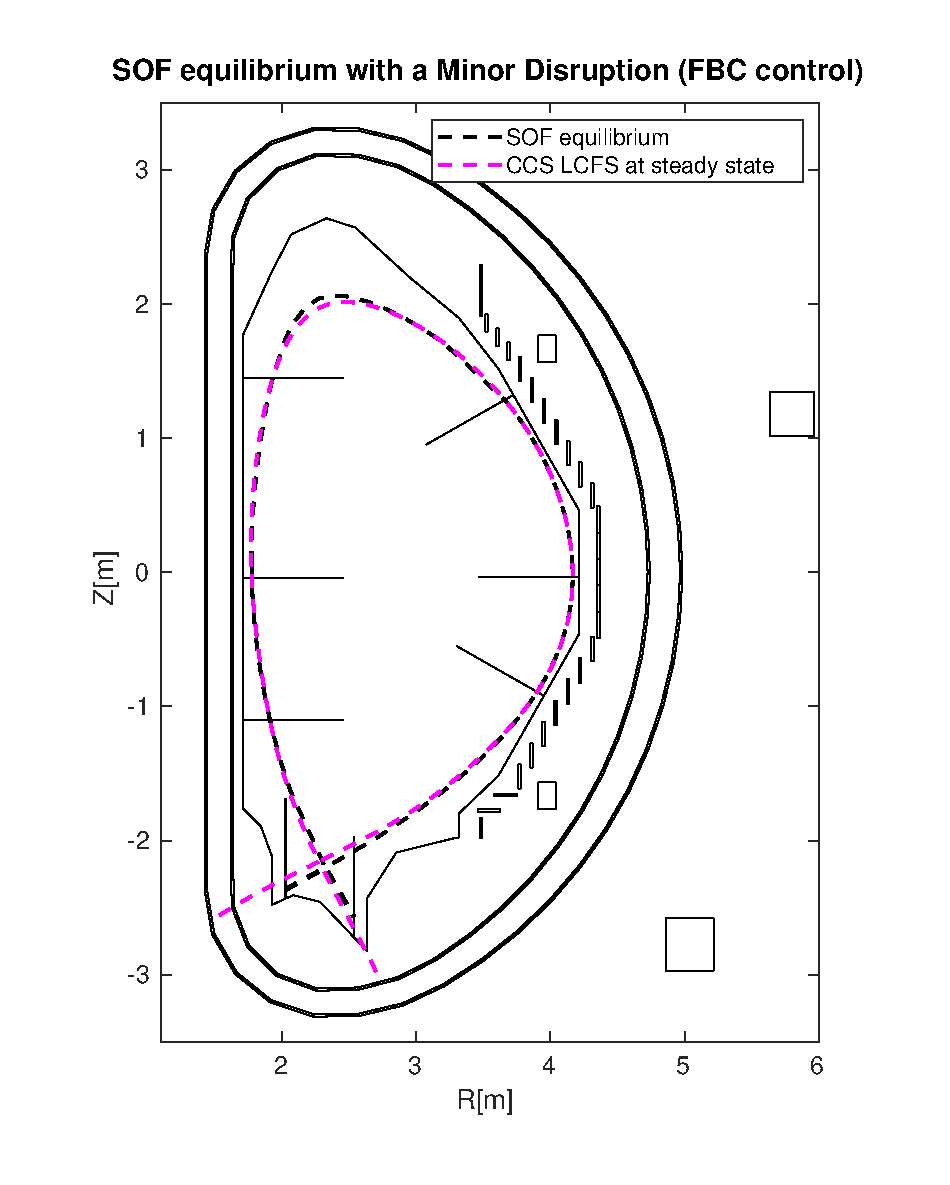
\includegraphics[height=8.75cm] {Chp3/Results_iso/8_gaps_mnr_disrp_equilVsLCFS_FBC.eps}  
			\caption{Comparison between the reference shape (i.e., the shape at the considered equilibrium) and the LCFS reconstructed by the CCS code at steady-state in the presence of a Minor disruption using the QST controller for the plasma shape and current and 8 control segments . 
				\label{FBS_isoflux_ss} }
		\end{subfigure}
		

\caption{ CREATE-NL JT60-SA Scenario~2 - SOF equilibrium compared with the LCFS reconstructed by the CCS method for 8 control points in the presence of a Minor disruption at steady-state using both the XSC and the QST control.  \label{compFBC_XSC_ss}}
\end{figure}




\begin{figure}[h]
	\centering
	\begin{subfigure}[b]{0.32\textwidth}
		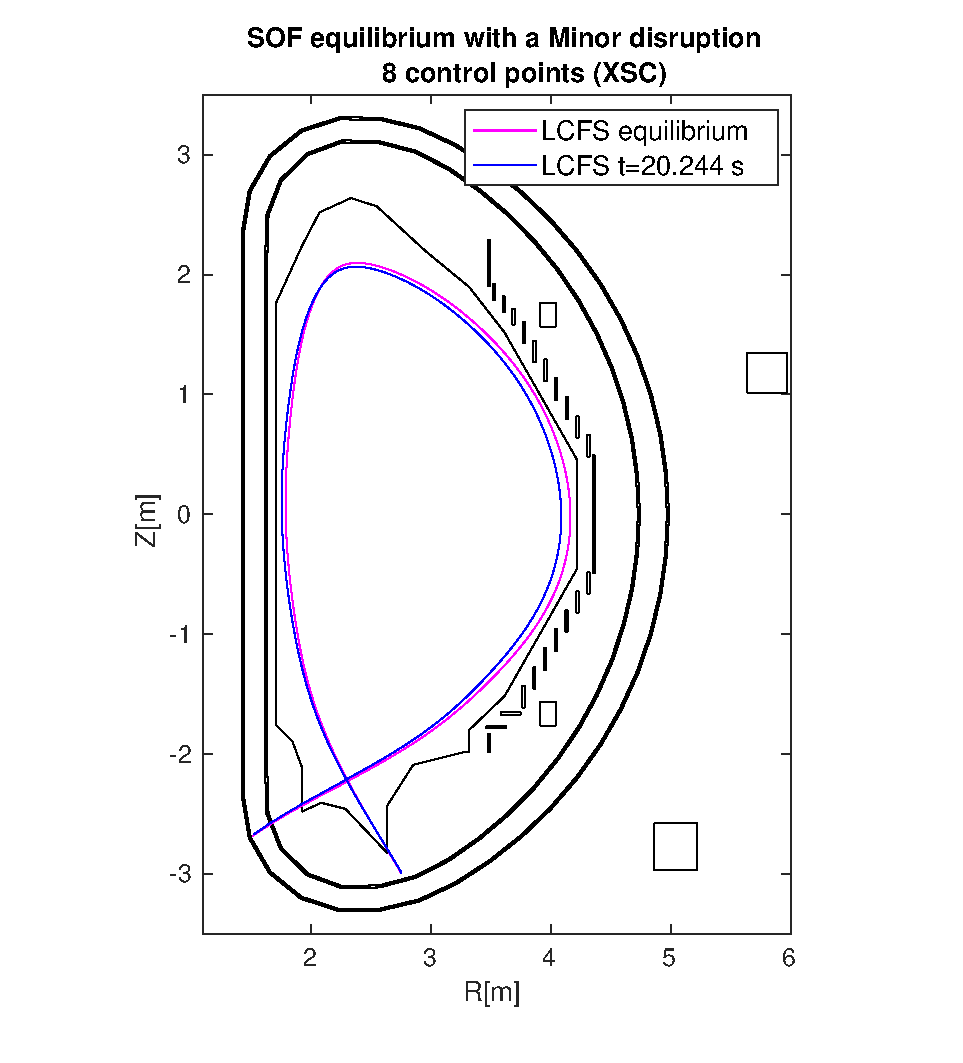
\includegraphics[height=8.75cm] {Chp3/Results_iso/8_gaps_mnr_disrp_20.244s.eps}  
		\caption{ Maximum deviation in plasma shape at t=20.244~s using the XSC for plasma shape.
			\label{XSC_20s} }
	\end{subfigure}
	%\quad 	\quad \quad \quad \quad
	\hspace{2 cm}
	\begin{subfigure}[b]{0.32\textwidth}
		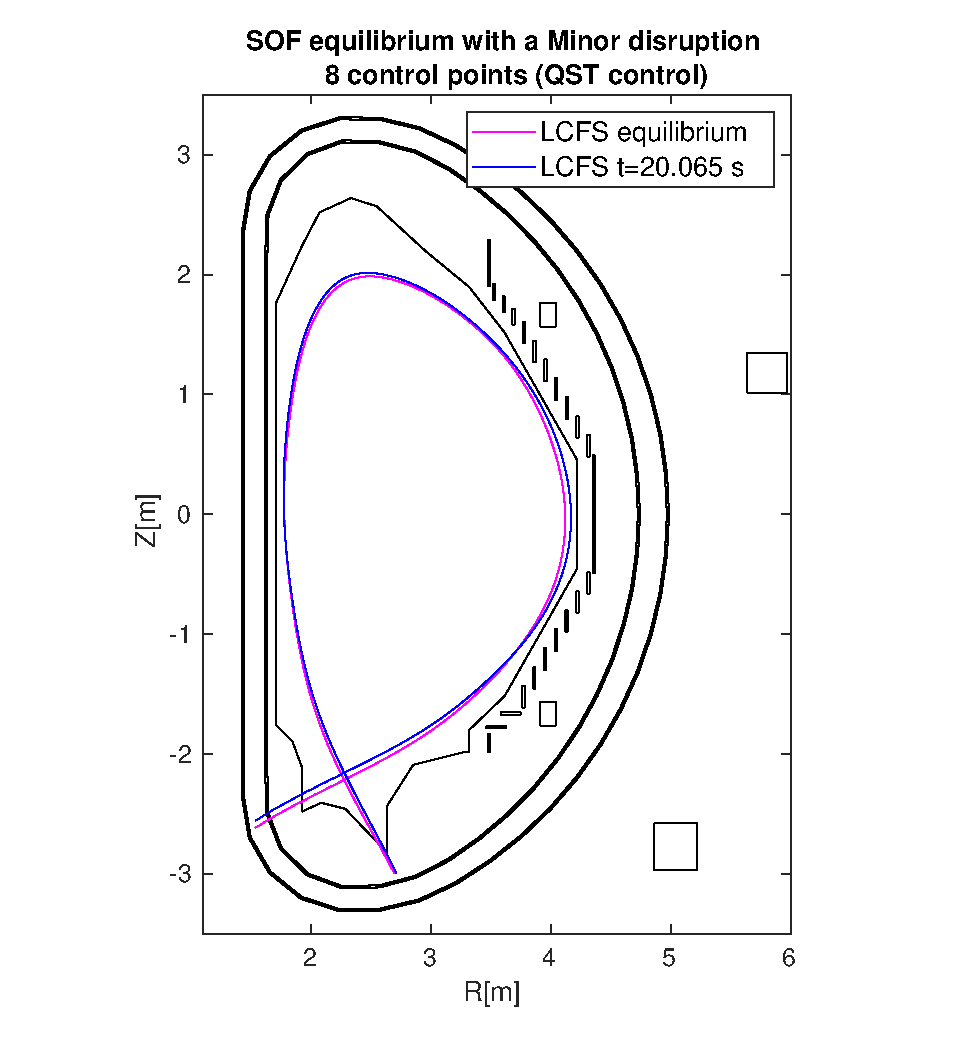
\includegraphics[height=8.75cm] {Chp3/Results_iso/8_gaps_mnr_disrp_20065sFBC.eps}  
		\caption{Maximum deviation in plasma shape at t=20.065~s using the QST control for plasma shape.
			\label{FBC_20s} }
	\end{subfigure}
	
	
	\caption{  CREATE-NL JT60-SA Scenario~2 - SOF equilibrium compared with the LCFS reconstructed by the CCS method for 8 control points in the presence of a Minor disruption (Disturbance ~ $\#3$) at the time of maximum deviation for both cases. As shown in figure ~\ref{MnrDisrp}, the disturbance occurs at $t~\sim 20 ~ s$  \label{20secs}}
\end{figure}



Figure~\ref{XpointFluxes} shows the time traces comparing the flux at the X-point and the 8 control points fluxes, for the XSC and the QST control cases. From these two graphs is noticeable that the QST controller takes around 0.5 ~s  more to reach the steady-state after the disturbance takes place than XSC , but the fluxes at the control points reach a state-state flux value way closer to the X-point flux than the fluxes using the  XSC for the simulation, in addition figure~\ref{FluxesError} shows the flux error time traces on the 8 control points for both controllers, on these plots is worth to mention that additionally to a smaller state-state error using the QST control, the maximum error values which are located right after the disturbance takes place are higher for the simulation using the XSC. 
\smallskip



%%Error plots

\begin{figure}[h]
	\centering
	\begin{subfigure}[b]{0.32\textwidth}
		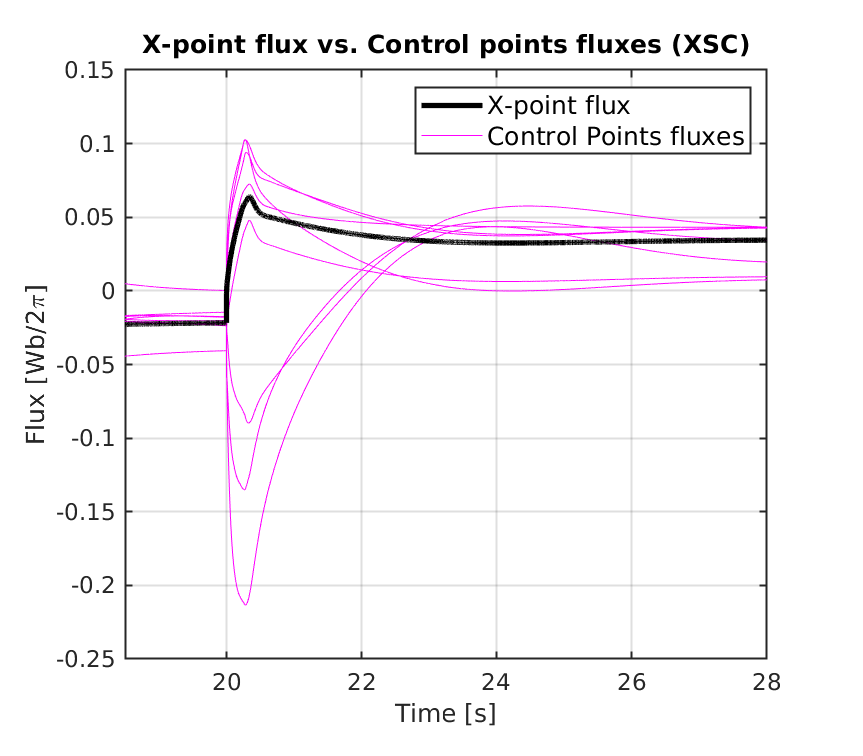
\includegraphics[height=6cm] {Chp3/Results_iso/8_gaps_XpointVSpoinsFlux_mnr_dsrp.eps}  
		\caption{ X-point flux compared to the control points fluxes using the XSC.
			\label{XpointVScntrlpointsXSC} }
	\end{subfigure}
	%\quad 	\quad \quad \quad \quad \qquad
	\hspace{2 cm}
	\begin{subfigure}[b]{0.32\textwidth}
		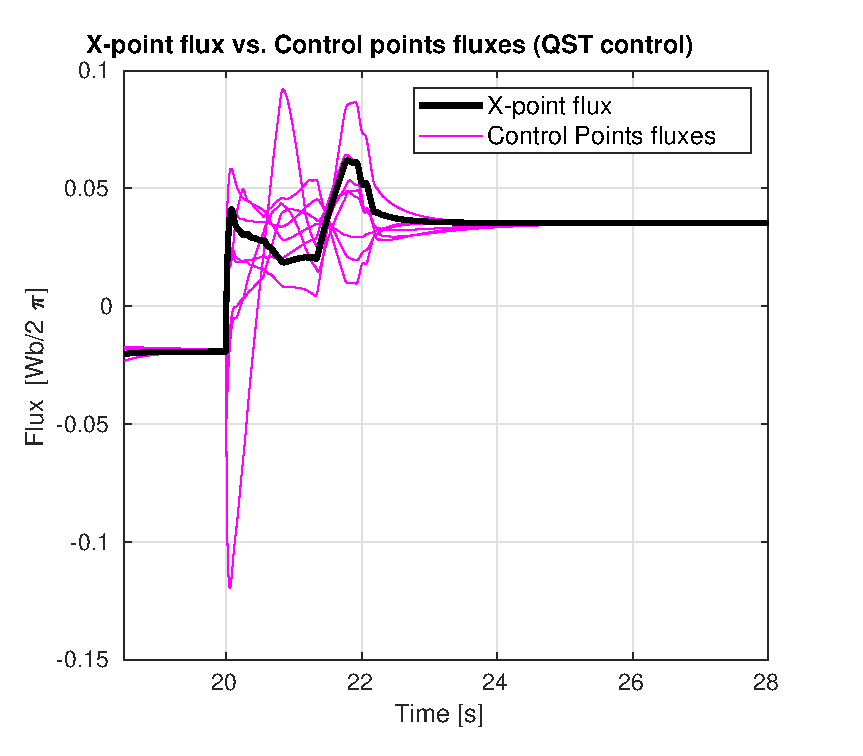
\includegraphics[height=6cm] {Chp3/Results_iso/8_gaps_Xpoint_flux_comparFBC.eps}  
		\caption{ X-point flux compared to the control points fluxes using the QST controller.
			\label{XpointVScntrlpointsFBC} }
	\end{subfigure}
\caption{Comparison between the flux at the X-point and the fluxes in the 8 control points reconstructed by the CCS method, when a Minor disruption is applaied at t=20 ~s using the XSC and the QST controller. It should be notice that QST control has a faster performance to reach the steady-state and less error. } \label{XpointFluxes}
\end{figure}


\begin{figure}[h]
	\centering
	\begin{subfigure}[b]{0.32\textwidth}
		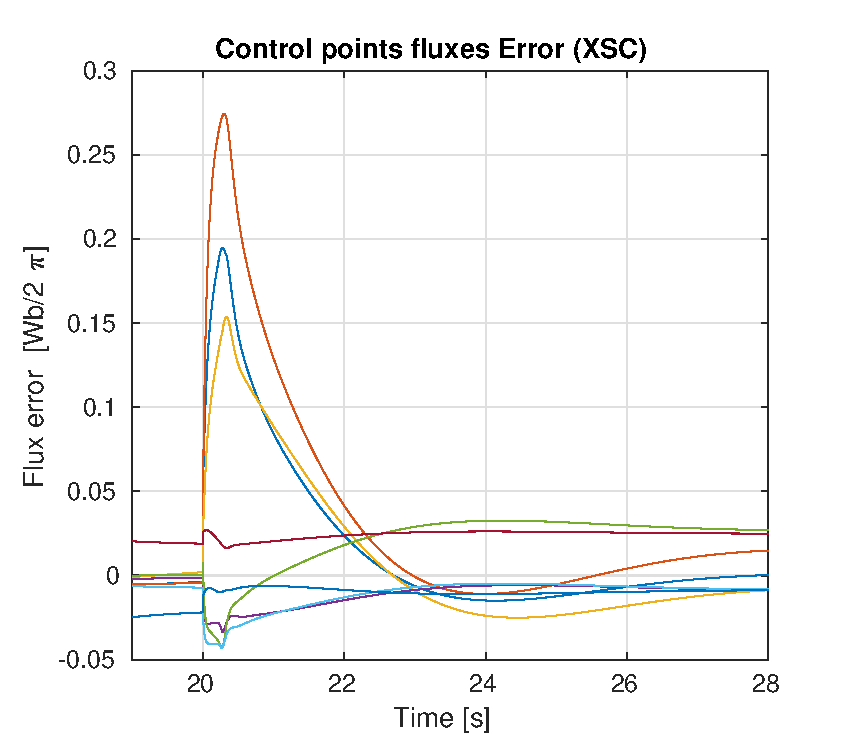
\includegraphics[height=5.5cm] {Chp3/Results_iso/8_gaps_fluxesError_mnr_dsrp.eps}  
		\caption{Flux errors using the XSC for 8 control points in the presence of a Minor disruption starting at $t=~20$.
			\label{FluxErrorXSC} }
	\end{subfigure}
	%\quad 	\quad \quad \quad \quad \quad
	\hspace{1 cm }
	\begin{subfigure}[b]{0.32\textwidth}
		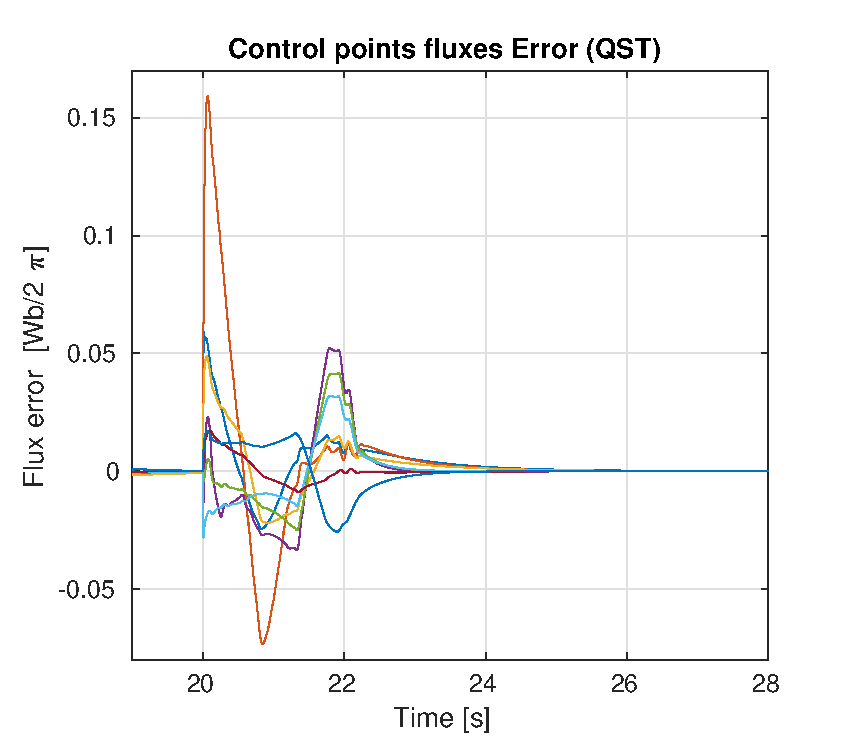
\includegraphics[height=5.5cm] {Chp3/Results_iso/8_gaps_fluxesError_mnr_dsrpFBC.eps}  
		\caption{ Flux errors using the QST controller for 8 control points in the presence of a Minor disruption starting  at $t=~20$.
			\label{FluxErroFBC} }
	\end{subfigure}
	
	\caption{Flux errors for the case of 8 control points in the presence of a Minor disruption using the XSC and the QST controller. Even though both controllers reject the disturbance, is possible to remark how the QST control has an overall smaller error.  }\label{FluxesError}
\end{figure}


In order to summarize all the results from the tested cases, tables~\ref{CCS_urano_Xpoint_error} , ~\ref{CCS_cmpELM_Xpoint_error} and ~\ref{CCS_mnr_Xpoint_error} outline the control points fluxes RMSE  and tables ~\ref{CCS_urano_Xpoint_error}, ~\ref{CCS_cmpELM_Xpoint_error} and ~\ref{CCS_mnr_Xpoint_error} present the X-point radial and vertical position errors in steady-state, these tables summarize results for all the different number of control points  with the three different disturbances. Some of the main aspects that are  possible to conclude from the tables results are :

\begin{enumerate}[label=(\alph*)]
	\item  For all disturbances the 8 control points selection has the biggest fluxes and X-point position steady-state errors while the cases with 19 control points the lesser ones.
	\item Disturbance $\#2$ (Compound ELM ) results present the lesser flux RMSE values in comparison with the other two disturbances. See table~\ref{fluxRMSE_cmpELM_table}.
	\item The simulations using the  QST controller present practically a flux RMSE equal to zero in steady-state for all disturbances while the XSC does not.
	\item For all the scenarios  the vertical XSC X-point error is  at least $~\%30$ greater  than the radial position error, while for the QST control the vertical position error tends to be around $~\%50$ lesser than the radial position.
	\item  As mentioned on the previous section and as it can be observe on the scheme in figure~\ref{JT60controlscheme}, the XSC isoflux approach also controls the X-point position, this is  noticeable for all the disturbances with 8 control points, where the vertical and horizontal position error values with the QST controller are at least ~$50 \%$ greater than the ones with the XSC .
	\item Despite the X-point control dynamics embedded on the XSC, for the 6 control points scenarios, the  radial X-point error positions are  similar between the XSC and the QST control simulations, and the vertical X-point error  using the XSC  is for all disturbances at least 10 times greater than the simulations with the QST controller.
\end{enumerate}




\begin{table}[]
	\centering
	\begin{tabular}{|l|c|c|c|c|}
		\hline
		\rowcolor{color2}
		\multicolumn{5}{|c|}{\textbf{Disturbance $\#1$ flux RMSE steady state      ~ ~ Wb/2$\pi$}}                                                                 \\ \hline
		\rowcolor{color1}
		Controller                 & \multicolumn{2}{c|}{eXtreme Shape Controller} & \multicolumn{2}{c|}{QST Controller}                 \\ \hline
		LCFS reconstruction method & CCS                   & CREATE                & CCS                      & CREATE                   \\ \hline
		6 points                   & 0.0116                & 0.0133                & $\sim 0$               & $\sim 0$                  \\ \hline
		8 points                   & 0.0166                & 0.0181                & $\sim 0$                 & $\sim 0$                  \\ \hline
		19 points                  & 0.0085                & 0.0088                & \cellcolor[HTML]{C0C0C0} & \cellcolor[HTML]{C0C0C0} \\ \hline
	\end{tabular}
	\caption{Steady-state flux RMSE values for the different selection of control points for  the JT60-SA scenario 2, SOF equilibrium in the presence of  Disturbance $\# 1$  at ~$t\sim 20 $~s. }
	\label{fluxRMS_Urano_table}
\end{table}

\begin{table}[h]
	\centering
	\begin{tabular}{|l|c|c|c|c|c|c|c|c|}
		\hline
		\rowcolor{color2}
		\multicolumn{9}{|c|}{\textbf{Disturbance $\#1$  steady state X-point position error}}                                                                                                                                                                         \\ \hline
		\rowcolor{color1}
		Controller                                                            & \multicolumn{4}{c|}{eXtreme Shape Controller}          & \multicolumn{4}{c|}{QST Controller}                                                                       \\ \hline
		\rowcolor{color3}
		\begin{tabular}[c]{@{}l@{}}LCFS reconstruction \\ method\end{tabular} & \multicolumn{2}{c|}{CCS} & \multicolumn{2}{c|}{CREATE} & \multicolumn{2}{c|}{CCS}                            & \multicolumn{2}{c|}{CREATE}                         \\ \hline
		& Rx~ mm       & Zx~ mm      & Rx~ mm        & Zx~ mm        & Rx~ mm                    & Zx ~mm                    & Rx~ mm                    & Zx ~mm                    \\ \hline
		6 points       &                                                       -4.606           & 19.96          & -3.576            & 28.16              & -1.434                        & -0.843                        & -1.16                        &   -0.316                      \\ \hline
		8 points                                                              &18.58          & 21.95          & 18.96            & 29.82           &   49.16                      &     -46.52                     & 59.66                       &           -40.92              \\ \hline
		19 points                                                             &2.62           & 12.84          & 2.375           & 20.51             & \cellcolor[HTML]{C0C0C0} & \cellcolor[HTML]{C0C0C0} & \cellcolor[HTML]{C0C0C0} & \cellcolor[HTML]{C0C0C0} \\ \hline
	\end{tabular}
	\caption{X-point position steady state error for  JT60-SA scenario 2, SOF equilibrium in the presence of  Disturbance $\# 1$ at ~$t\sim 20 $~s . The XSC and  QST controller were used in different simulations for the shape control along  with two reconstruction methods for the LCFS. }
	\label{CCS_urano_Xpoint_error}
\end{table}



\begin{table}[]
	\centering
	\begin{tabular}{|l|c|c|c|c|}
		\hline
		\rowcolor{color2}
		\multicolumn{5}{|c|}{\textbf{Disturbance $\#2$ (Compound ELM) flux RMSE steady state      ~ ~ Wb/2$\pi$}}                                                                 \\ \hline
		\rowcolor{color1}
		Controller                 & \multicolumn{2}{c|}{eXtreme Shape Controller} & \multicolumn{2}{c|}{QST Controller}                 \\ \hline
		LCFS reconstruction method & CCS                   & CREATE                & CCS                      & CREATE                   \\ \hline
		6 points                   & 0.0014                & 0.0022                & $\sim 0$               & $\sim 0$                  \\ \hline
		8 points                   & 0.0104                & 0.0101                & $\sim 0$                 & $\sim 0$                  \\ \hline
		19 points                  & 0.0023                & 0.0028                & \cellcolor[HTML]{C0C0C0} & \cellcolor[HTML]{C0C0C0} \\ \hline
	\end{tabular}
	\caption{Steady-state flux RMSE values for the different selection of control points for  the JT60-SA scenario 2, SOF equilibrium in the presence of  Disturbance $\# 2$ (Compound ELM) at ~$t\sim 20 $~s. }
	\label{fluxRMSE_cmpELM_table}
\end{table}

\begin{table}[]
	\centering
	\begin{tabular}{|l|c|c|c|c|c|c|c|c|}
		\hline
		\rowcolor{color2}
		\multicolumn{9}{|c|}{\textbf{Disturbance $\#2$ (Compound ELM)  steady state X-point position error}}                                                                                                                                                                         \\ \hline
		\rowcolor{color1}
		Controller                                                            & \multicolumn{4}{c|}{eXtreme Shape Controller}          & \multicolumn{4}{c|}{QST Controller}                                                                       \\ \hline
		\rowcolor{color3}
		\begin{tabular}[c]{@{}l@{}}LCFS reconstruction \\ method\end{tabular} & \multicolumn{2}{c|}{CCS} & \multicolumn{2}{c|}{CREATE} & \multicolumn{2}{c|}{CCS}                            & \multicolumn{2}{c|}{CREATE}                         \\ \hline
		& Rx~ mm       & Zx~ mm      & Rx~ mm        & Zx~ mm        & Rx~ mm                    & Zx ~mm                    & Rx~ mm                    & Zx ~mm                    \\ \hline
		6 points       &                                                       0.3968           & -2.455          & 1.3            & 2.556              & -0.481                        & -0.267                        & -0.019                       &   0.0143                     \\ \hline
		8 points                                                              &15.72          & -8.41          & 16.61            & -3.098           &   50.18                     &     -43.25                     & 54.44                      &           -32.68             \\ \hline
		19 points                                                             &-0.0007           & 0.0237          & -0.1916          & -4.69             & \cellcolor[HTML]{C0C0C0} & \cellcolor[HTML]{C0C0C0} & \cellcolor[HTML]{C0C0C0} & \cellcolor[HTML]{C0C0C0} \\ \hline
	\end{tabular}
	\caption{X-point position steady state error for  JT60-SA scenario 2, SOF equilibrium in the presence of  Disturbance $\# 2$ (Compound ELM) at ~$t\sim 20 $~s . The XSC and  QST controller were used in different simulations for the shape control along  with two reconstruction methods for the LCFS. }
	\label{CCS_cmpELM_Xpoint_error}
\end{table}




\begin{table}[]
	\centering
	\begin{tabular}{|l|c|c|c|c|}
		\hline
		\rowcolor{color2}
		\multicolumn{5}{|c|}{\textbf{Disturbance $\#3$ (Minor disruption) flux RMSE steady state      ~ ~ Wb/2$\pi$}}                                                                 \\ \hline
		\rowcolor{color1}
		Controller                 & \multicolumn{2}{c|}{eXtreme Shape Controller} & \multicolumn{2}{c|}{QST Controller}                 \\ \hline
		LCFS reconstruction method & CCS                   & CREATE                & CCS                      & CREATE                   \\ \hline
		6 points                   & 0.0121                & 0.0139                & $\sim 0$               & $\sim 0$                  \\ \hline
		8 points                   & 0.0152                & 0.0170                & $\sim 0$                 & $\sim 0$                  \\ \hline
		19 points                  & 0.0069                & 0.0088                & \cellcolor[HTML]{C0C0C0} & \cellcolor[HTML]{C0C0C0} \\ \hline
	\end{tabular}
	\caption{Steady-state flux RMSE values for the different selection of control points for  the JT60-SA scenario 2, SOF equilibrium in the presence of  Disturbance $\# 3$ (Minor disruption) at ~$t\sim 20 $~s. }
	\label{fluxRMSE_mnr_table}
\end{table}





\begin{table}[]
	\centering
	\begin{tabular}{|l|c|c|c|c|c|c|c|c|}
		\hline
			\rowcolor{color2}
		\multicolumn{9}{|c|}{\textbf{Disturbance $\#3$ (Minor disruption) steady state X-point position error}}                                                                                                                                                                         \\ \hline
			\rowcolor{color1}
		Controller                                                            & \multicolumn{4}{c|}{eXtreme Shape Controller}          & \multicolumn{4}{c|}{QST Controller}                                                                       \\ \hline
			\rowcolor{color3}
		\begin{tabular}[c]{@{}l@{}}LCFS reconstruction \\ method\end{tabular} & \multicolumn{2}{c|}{CCS} & \multicolumn{2}{c|}{CREATE} & \multicolumn{2}{c|}{CCS}                            & \multicolumn{2}{c|}{CREATE}                         \\ \hline
		& Rx~ mm       & Zx~ mm      & Rx~ mm        & Zx~ mm        & Rx~ mm                    & Zx ~mm                    & Rx~ mm                    & Zx ~mm                    \\ \hline
		6 points       &                                                       -4.92           & 20.9          & -3.57            & 28.8              & -2.70                        & -0.105                        & -2.24                        &   0.369                      \\ \hline
		8 points                                                              &17.44           & 21.56          & 17.81            & 29.04           &   47.08                      &     -46.56                     & 57.61                       &           -41.42              \\ \hline
		19 points                                                             &-5.54           & 16.78          & -4.42           & 24.41             & \cellcolor[HTML]{C0C0C0} & \cellcolor[HTML]{C0C0C0} & \cellcolor[HTML]{C0C0C0} & \cellcolor[HTML]{C0C0C0} \\ \hline
	\end{tabular}
\caption{X-point position steady state error for  JT60-SA scenario 2, SOF equilibrium in the presence of  Disturbance $\# 3$ (Minor disruption) at ~$t\sim 20 $~s . The XSC and  QST controller were used in different simulations for the shape control along  with two reconstruction methods for the LCFS.  }
\label{CCS_mnr_Xpoint_error}
\end{table}






\subsection{Shape reference change}

A change in the plasma shape for the Scenario~2 - SOF equilibrium has been also considered. In this test scenario closed-loop simulations  with the  CCS reconstruction method and the isoflux XSC for the plasma shape were performed.   Since the configuration with 8 control points seems to be for all cases the one most challenging due to the error values in steady-state obtained on the past subsection, these selection of control points was used for this simulation. The transition time from the initial shape to the target was set equal to 1.5 ~s.  Figure ~\ref{sqzd} shows the equilibrium LCFS (Scenario~2 -SOF), the desired target shape and the LCFS at steady state reconstructed by the CCS method. It can be noticed that the controller is able to track the required shape with negligible error at steady-state, taking $\sim 6~ s$ to reach to it. Figure~\ref{FluxesSqzd} shows the time traces for the fluxes at the 8 control points compared with the X-point flux and figure~\ref{errorFluxessqzd} shows the correspondent control flux errors.



\begin{figure}
	\begin{center}
		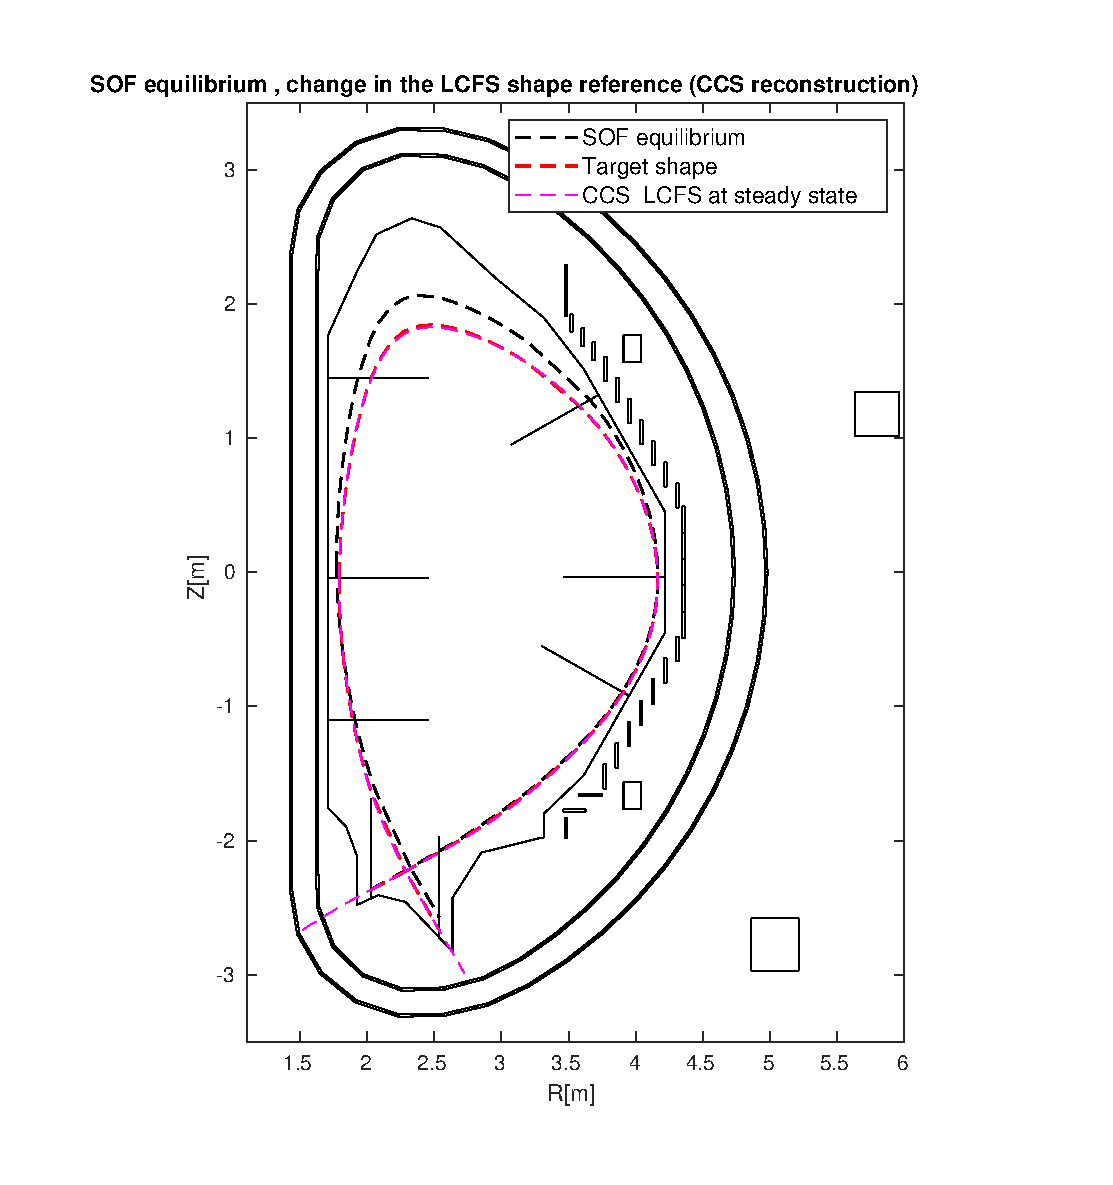
\includegraphics[width=0.7\textwidth]{Chp3/8gaps_LCFScompar_sqzd.eps}
	\end{center}	
\caption{XSC isoflux response to a change of shape request. The dashed black shape is the starting shape, while the red one is the target shape. The magenta dashed shape is the LCFS at steady state.  }
	\label{sqzd}
\end{figure}



\begin{figure}
	\begin{center}
		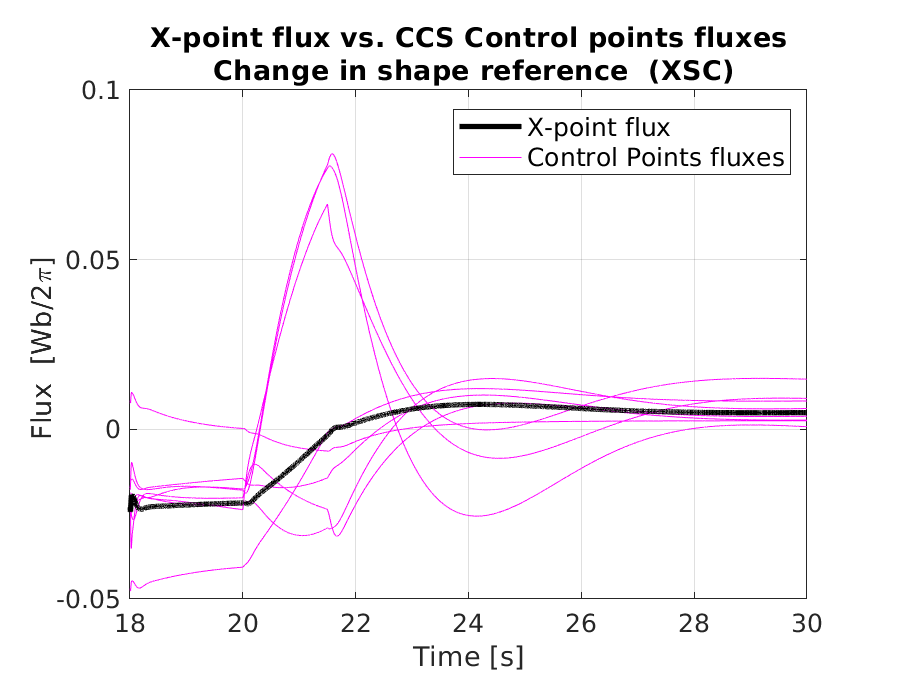
\includegraphics[width=0.6\textwidth]{Chp3/8_gaosXpointVSpoinsFlux_sqzd.eps}
	\end{center}	
	\caption{Comparison between the flux at the X-point and the fluxes a }
	\label{FluxesSqzd}
\end{figure}


\begin{figure}
	\begin{center}
		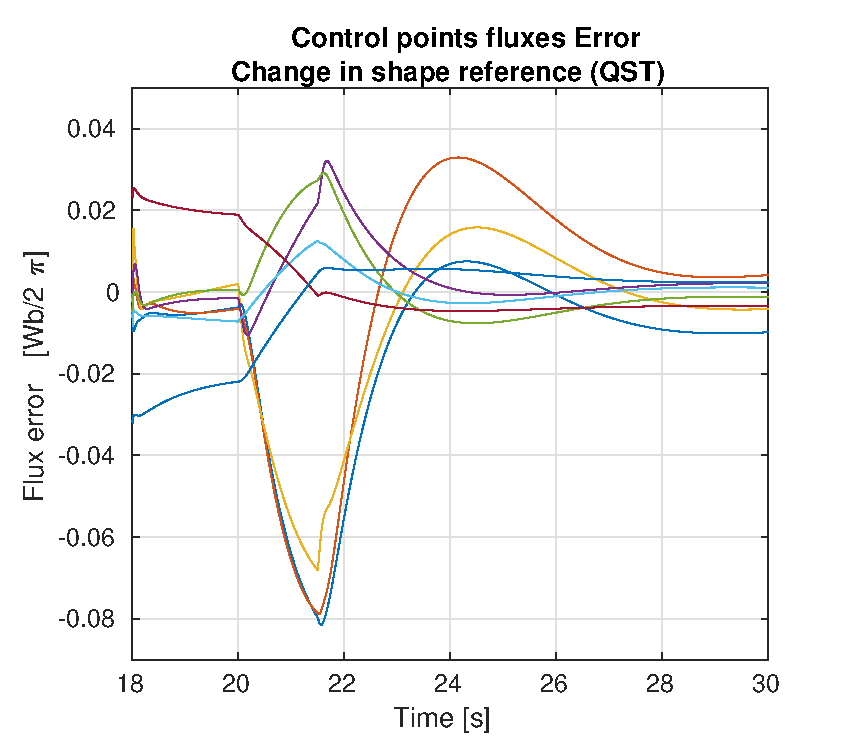
\includegraphics[width=0.6\textwidth]{Chp3/8_gaps_fluxesError_sqzd.eps}
	\end{center}	
	\caption{ Flux control error for the case of 8 control points for a change in the shape reference  between 20 and 21.5 $s $.}
	\label{errorFluxessqzd}
\end{figure}
